% \documentclass[nofootinbib,english, aip, jcp, priprint, graphicx,floatfix]{revtex4-1}
\documentclass[12pt, nofootinbib,english, amsmath, amssymb, aps, priprint, graphicx,floatfix]{revtex4-1}
\usepackage{amsmath,bm}
\usepackage{amsthm}
\usepackage{amssymb}
\usepackage{mathrsfs}
\usepackage{bbm,latexsym}
\usepackage{graphicx}
\usepackage{cancel}
\usepackage{enumitem}
\usepackage{wrapfig}
\usepackage{setspace}
\usepackage[bottom]{footmisc}

%%%%%%%%%% Start TeXmacs macros
\newcommand{\mathd}{\mathrm{d}}
\newcommand{\nin}{\not\in}
\newcommand{\tmop}[1]{\ensuremath{\operatorname{#1}}}

\newcommand{\theepsrate}{\varepsilon + \sqrt{\varepsilon/2}}
\newcommand{\tmtextbf}[1]{{\bfseries{#1}}}
\newtheorem{definition}{Definition}
\newtheorem{proposition}{Proposition}
\newtheorem*{proposition*}{Proposition}
\newtheorem*{corollary*}{Corollary}
\newtheorem*{corollary}{Corollary}
\newtheorem{theorem}{Theorem}
\newtheorem{lemma}{Lemma}
\newtheorem{algorithm}{Algorithm}
%%%%%%%%%% End TeXmacs macros

% \draft % marks overfull lines with a black rule on the right

\theoremstyle{plain}
\newtheorem{thm}{\protect\theoremname}
\newtheorem*{thm*}{\protect\theoremname}
\newtheorem*{lem*}{\protect\lemmaname}
\theoremstyle{definition}
\newtheorem{defn}[thm]{\protect\definitionname}
\theoremstyle{plain}
\newtheorem{cor}[thm]{\protect\corollaryname}

\newcommand{\normal}{{\mathfrak{n}}}
\newcommand{\TODOTHIS}{{\huge !!!!}}
\newcommand{\indicatorf}[1]{\mathbb{I}_{#1}}
\newcommand{\capac}[2]{\ensuremath{\operatorname{cap}}(#1,#2)}
\newcommand{\hausdorffmeasure}{\mathscr{H}(dx)}
\newcommand{\PMeasure}{\mathscr{P}(dx)}
\newcommand{\tPMeasure}{\tilde{\mathscr P}(dx)}
\newcommand{\fnsp}{\mathscr{H}^1}
\newcommand{\bb}[1]{\mathcal{B}\left(#1\right)}
\newcommand{\BB}[1]{\mathcal{\bar B}\left(#1\right)}


\usepackage[english]{babel}
\providecommand{\corollaryname}{Corollary}
\providecommand{\propositionname}{Proposition}
\providecommand{\definitionname}{Definition}
\providecommand{\lemmaname}{Lemma}
\providecommand{\theoremname}{Theorem}

\newcommand{\dA}{{\dot A}}
\newcommand{\tA}{{\tilde A}}
\newcommand{\dB}{{\dot B}}
\newcommand{\tB}{{\tilde B}}
\newcommand{\capA}{\kappa_A}
\newcommand{\capB}{\kappa_B}

\parskip=1pt
\usepackage[compact]{titlesec}
\titlespacing{\section}{0pt}{20pt}{20pt}
\titlespacing{\subsection}{0pt}{*0}{*0}
\titlespacing{\subsubsection}{0pt}{*0}{*0}

\begin{document}

\title{Efficiently Computing First Passage Probabilities Using First Passage Capacities} %Title of paper

\author{Jackson Loper}
\thanks{These two authors contributed equally}
\affiliation{Data Science Institute, Columbia University, New York, NY, USA}

\author{Guangyao Zhou}
\thanks{These two authors contributed equally}

\author{Stuart Geman}

\affiliation{Division of Applied Mathematics, Brown University, Providence, RI, USA}
\date{\today}

\begin{abstract}
	A reversible stochastic differential equation is initialized at position $x_0$ -- where will it go next?  What is the probability it will reach one target before it reaches another target?  We here propose an approach for estimating this probability.  We focus on the situation that it takes a long time to hit any target; in this case direct simulation of the hitting probabilities becomes prohibitively expensive.  We turn this curse into a blessing; if the timescales are sufficiently long the system will essentially ``forget'' its initial condition before it hits any target.  In this case we show that the hitting probabilities can be accurately approximated using only local simulations around each target, obviating the need for global simulations.  In empirical tests, we find that these estimates can be computed in the same time it would take to compute a single direct simulation, but they achieve the same accuracy as would be obtained from one hundred simulations.
\end{abstract}

\pacs{}% insert suggested PACS numbers in braces on next line

\maketitle %\maketitle must follow title, authors, abstract and \pacs

\section{Introduction}
\label{sec:Introduction}

Reversible diffusions play a key role in a wide variety of physical systems.  For example, the folding of macromolecules into their native configurations is often posed as a diffusion (either directly through simulations of atomic dynamics or indirectly through mesoscopic models \cite{Scheraga2007-qw,Hospital2015-ol,lei2010direct}), the fluctuation of chemical species in solution can be modeled as diffusions (``chemical Langevin equations'' are one classic example of this approach \cite{sotiropoulos2011analytical,gillespie2000chemical}), the motion of particles through membranes can be posed as a diffusion \cite{holcman2004escape}, and so-on.   In all cases, the the physical state of the system at time $t$ is represented through a variable $X_t$, and this variable evolves according to a stochastic differential equation. 

In this paper we seek to estimate first-passage hitting probabilities of such diffusions: given an initial condition $X_0$ and two targets, $A,B$, what is the probability that we will hit target $A$ first?   Here each target represents a set of physical configurations.  For example, if $X$ represents the position of a particle trapped inside a sphere with two holes, $A$ and $B$ might represent the two holes.  The hitting probability then indicates the probability that the particle exits through the first hole.  These probabilities are also sometimes called ``splitting probabilities'' \cite{E2006-fm}.  This paper develops a new algorithm for approximating these hitting probabilities.

The algorithm proposed in this paper is designed for cases where the diffusion can ``forget'' its initial condition before either target is hit.  To make this idea rigorous, we need three ingredients:
\begin{itemize}
    \item the initial configuration $X_0$ must lie \emph{inside} a set of physical configurations we denote $M$
    \item the targets $A$ and $B$ lie \emph{outside} the set $M$
    \item the first passage time out of $M$ is long (a long time elapses before the process exits the set $M$)
\end{itemize}
This last condition is vague -- how long is long enough?  A simplistic answer is that the proposed algorithm will be more accurate when the first passage time is longer.  A more precise answer requires some machinery from the theory of ergodicity.  Recall that reversible diffusions are ergodic: as time goes on, it gets harder and harder to guess the initial condition from it's final configuration.  As this happens, the process is said to become ``mixed,'' and the speed with which the initial condition is forgotten is called the ``mixing rate.''  If the first passage time out of $M$ is long relative to this mixing rate, the hitting probability will be nearly the same no matter which initial condition we started from.  It is this property we actually need: if the hitting probability varies by at most $\varepsilon$ among all initial conditions inside the set $M$, the proposed algorithm's approximation error is less than $\varepsilon + \sqrt{\varepsilon/2}$.  Figure \ref{fig:ToyModel} gives a rough sketch of this idea.  Rigorous definitions are given in  \S\ref{sec:Preliminaries}.  

Are there any real cases where the diffusion can forget its initial condition in this way?  The narrow-escape literature gives at least one class of examples.  In these examples $X$ is a Brownian motion trapped inside a set by reflecting boundaries, and the targets are very small windows in boundary of the sphere.  These models have been successfully applied to a variety of mesoscopic biosystems (cf. \cite{schuss2007narrow} and the references therein).  These kinds of diffusions may also be relevant for modeling the folding of large molecules.  TCB McLeish has said that ``folding rates are controlled by the rate of diffusion of pieces of the open coil in their search for favorable contacts'' \cite{McLeish2005-dq}.  There is also some experimental evidence that the exploration of large regions is the rate-limiting step for a variety of processes \cite{Goldberg1999-mv,Jacob1999-bs,Plaxco1998-iv,Wales2006-ur}.  If these results bear out, the first-passage time out of this exploration may be long and our conditions may hold. 

Many standard methods for calculating hitting probabilities fail for diffusions of this kind.  When the escape time from $M$ is large, the associated partial differential equations often include large Lipschitz constants and direct Monte-Carlo simulation requires prohibitive number of timesteps (cf.\ \cite{Baum1986-we, Wille1987-tf, Machta2009-gh}).  Some authors take a pessimistic view on this subject: ``If these processes are intrinsically slow, i.e. require an extensive sampling of state space, not much can be done to speed up their simulation without destroying the dynamics of the system'' \cite{Christen2008-ge}.

In fact, diffusions of this kind enjoy certain properties which actually make analysis easier.  The literature includes a variety of tools which use such properties to advantage.  Here we review a few of these tools:

\begin{description}
    \item[Analytic analyses] When the targets are very small, the first passage hitting times are often well-approximated by analytic formulae.  The narrow-escape literature has developed many techniques in this direction.  Much of this literature focuses on making these formulas as accurate as possible for specific geometric configurations, such as the case of $N$ circular targets (cf.\ \cite{cheviakov2010asymptotic}), the case that one target lies at the end of a long tube (cf.\ \cite{li2014matched}), or the case that the motion is trapped inside a symmetric domain (cf.\ \cite{Chevalier2010-bq,Condamin2006-vi,Coombs2009-pe,Lindsay2017-ds}).  There is also some work on efficient numerical methods for low-dimensional problems using insights from these analytic results (cf.\ \cite{kaye2019fast}).  Note that this literature mostly focuses on hitting times, whereas in this paper we focus on hitting probabilities.   However, the first-passage probabilities are nearly inversely proportional to the mean first-passage times for many cases, so these techniques can often be used to estimate first-passage probabilities.  A helpful overview of many of the main ideas in this literature can be found in \cite{Benichou2014-jb}.

    \item[Markov State Models] Markov State Models (MSM) begin by partitioning the state-space of the diffusion into $n$ sets (``states'').  The diffusion can be understood at a coarse level by looking at which state the process is in at any given time (cf.\ \cite{Pande2010-yi, Chodera2014-bh, Husic2018-xp}).   In some cases the time it takes to move between states is long relative to the rate of mixing inside the states.  This separation of timescales ensures that the coarse process is approximately Markovian.  We can therefore approximately simulate the discrete process as long as we know the distribution on the exit times and the probability of transitioning to each possible state.  The amount of computational time required to simulate from this approximate process does not depend upon how long the process actually spends in each state.

    \item[Site-localizing functions] Site-localizing functions take a relaxed version of the MSM idea; instead of creating a hard partitioning of the space, one constructs basis functions $g_1(x)\cdots g_n(x)$ such that $\sum_i g_i(x)=1$.  In many cases the action of the relevant infinite-dimensional diffusion operators can be well-approximated by the their action on the $n$-dimensional space spanned by these basis functions.   For example, under a separation-of-timescales assumption, Morro (cf.\ \cite{moro1995kinetic}) shows a way to design basis functions which faithfully represent the diffusion's behavior on the slow timescale.

    \item[Milestoning] In some cases it is possible to construct a low-dimensional reaction coordinate which measures the distance from the targets in some suitable metric.  In some cases the movement along this reaction coordinate is slow relative to the mixing rate along all other directions.  This separation of timescales ensures that the dynamics of the diffusion along this coordinate are approximately Markovian.  If the reaction coordinate is carefully chosen, many properties of the original diffusion are maintained in this low-dimensional projection \cite{E2006-fm}.  Simulating from this low-dimensional approximate diffusion can yield useful insight into the overall behavior \cite{Bello-Rivas2015-ld}.  
\end{description}

All of the ideas above take advantage of some kind of separation of timescales.  In this paper we investigate a new algorithm which uses separated timescales.  

We here give a high-level summary of the mathematics behind the algorithm; a more detailed exposition can be found in \S\ref{sec:MainResults}.  Let $h(x)$ denote the chance the diffusion arrives in set $A$ before set $B$ when it is initialized at configuration $x$.  Recall that $h$ can be understood as the solution of a variational problem (we review this matter in Appendix \ref{sec:three_perspectives}).  The true solution of the variational problem, $h$, is a function that varies continuously as a function of the initial condition $x$.  However, we can solve the variational problem under the forced assumption that the hitting probability is exactly the same for every initial condition in a set $M$.  In particular, we will assume there is some $\bar h \in \mathbb{R}$ such that $h(x)=\bar h$ for every $x \in M$.   In Theorem \ref{thm:main_thm}, we show that we can control the error introduced by this forced assumption: $|\bar h - h(x) |\leq \varepsilon + \sqrt{\varepsilon/2}$, where $\varepsilon$ is the true difference between the maximum and minimum hitting probabilities for initial conditions in $M$.  Under this forced assumption the variational problem becomes much easier to solve; the value of $\bar h$ depends only on the dynamics outside of $M$, and this dependency can be summarized through what we call ``first passage capacities.''  These capacities can be calculated using integrals around a neighborhood of each target.  

In brief, one can efficiently compute first-passage capacities around each target and use these capacities to get good estimates of the hitting probabilities.  The key advantage of this approach is that it allows us to get good estimates while completely ignoring all dynamics inside $M$.  This is particularly valueable if $M$ is a large, high-dimensional set.  When $M$ is very large, it is unclear how one would partition $M$, making Markov State Models difficult to implement.  Similarly it is unclear how one should formulate a reaction coordinate, making milestoning approaches difficult to implement.  Integrating over all of $M$ is computationally burdensome in this case, making site-localizing functions difficult to implement.  Asymptotic techniques from the narrow escape/reaction-controlled diffusion literature may still be applied, but only if the problem falls into one of the very specific cases which have already been studied.  Most of these cases lie in two or three-dimensions, feature regular targets, and assume the diffusion has no energetic potential.  By contrast, first passage capacities can be calculated efficiently for a diffusion with an arbitrary energetic potential, target shape, and ambient dimension.  Moreover, first-passage capacities are fundamentally non-asymptotic quantities; for any problem the approximation error is bounded explicitly in terms of the extent to which the hitting probability varies inside $M$, i.e. $\varepsilon$.   First-passage capacities do come with a significant limitation, however: they do not give direct insight into the overall timescale of the diffusion. There is an overall proportionality constant which connects first-passage hitting probabilities to the first-passage hitting times, and this constant cannot be recovered from the first-passage capacities.  We discuss this limitation further in \S\ref{sec:Discussion}.

\begin{figure}
    \centering  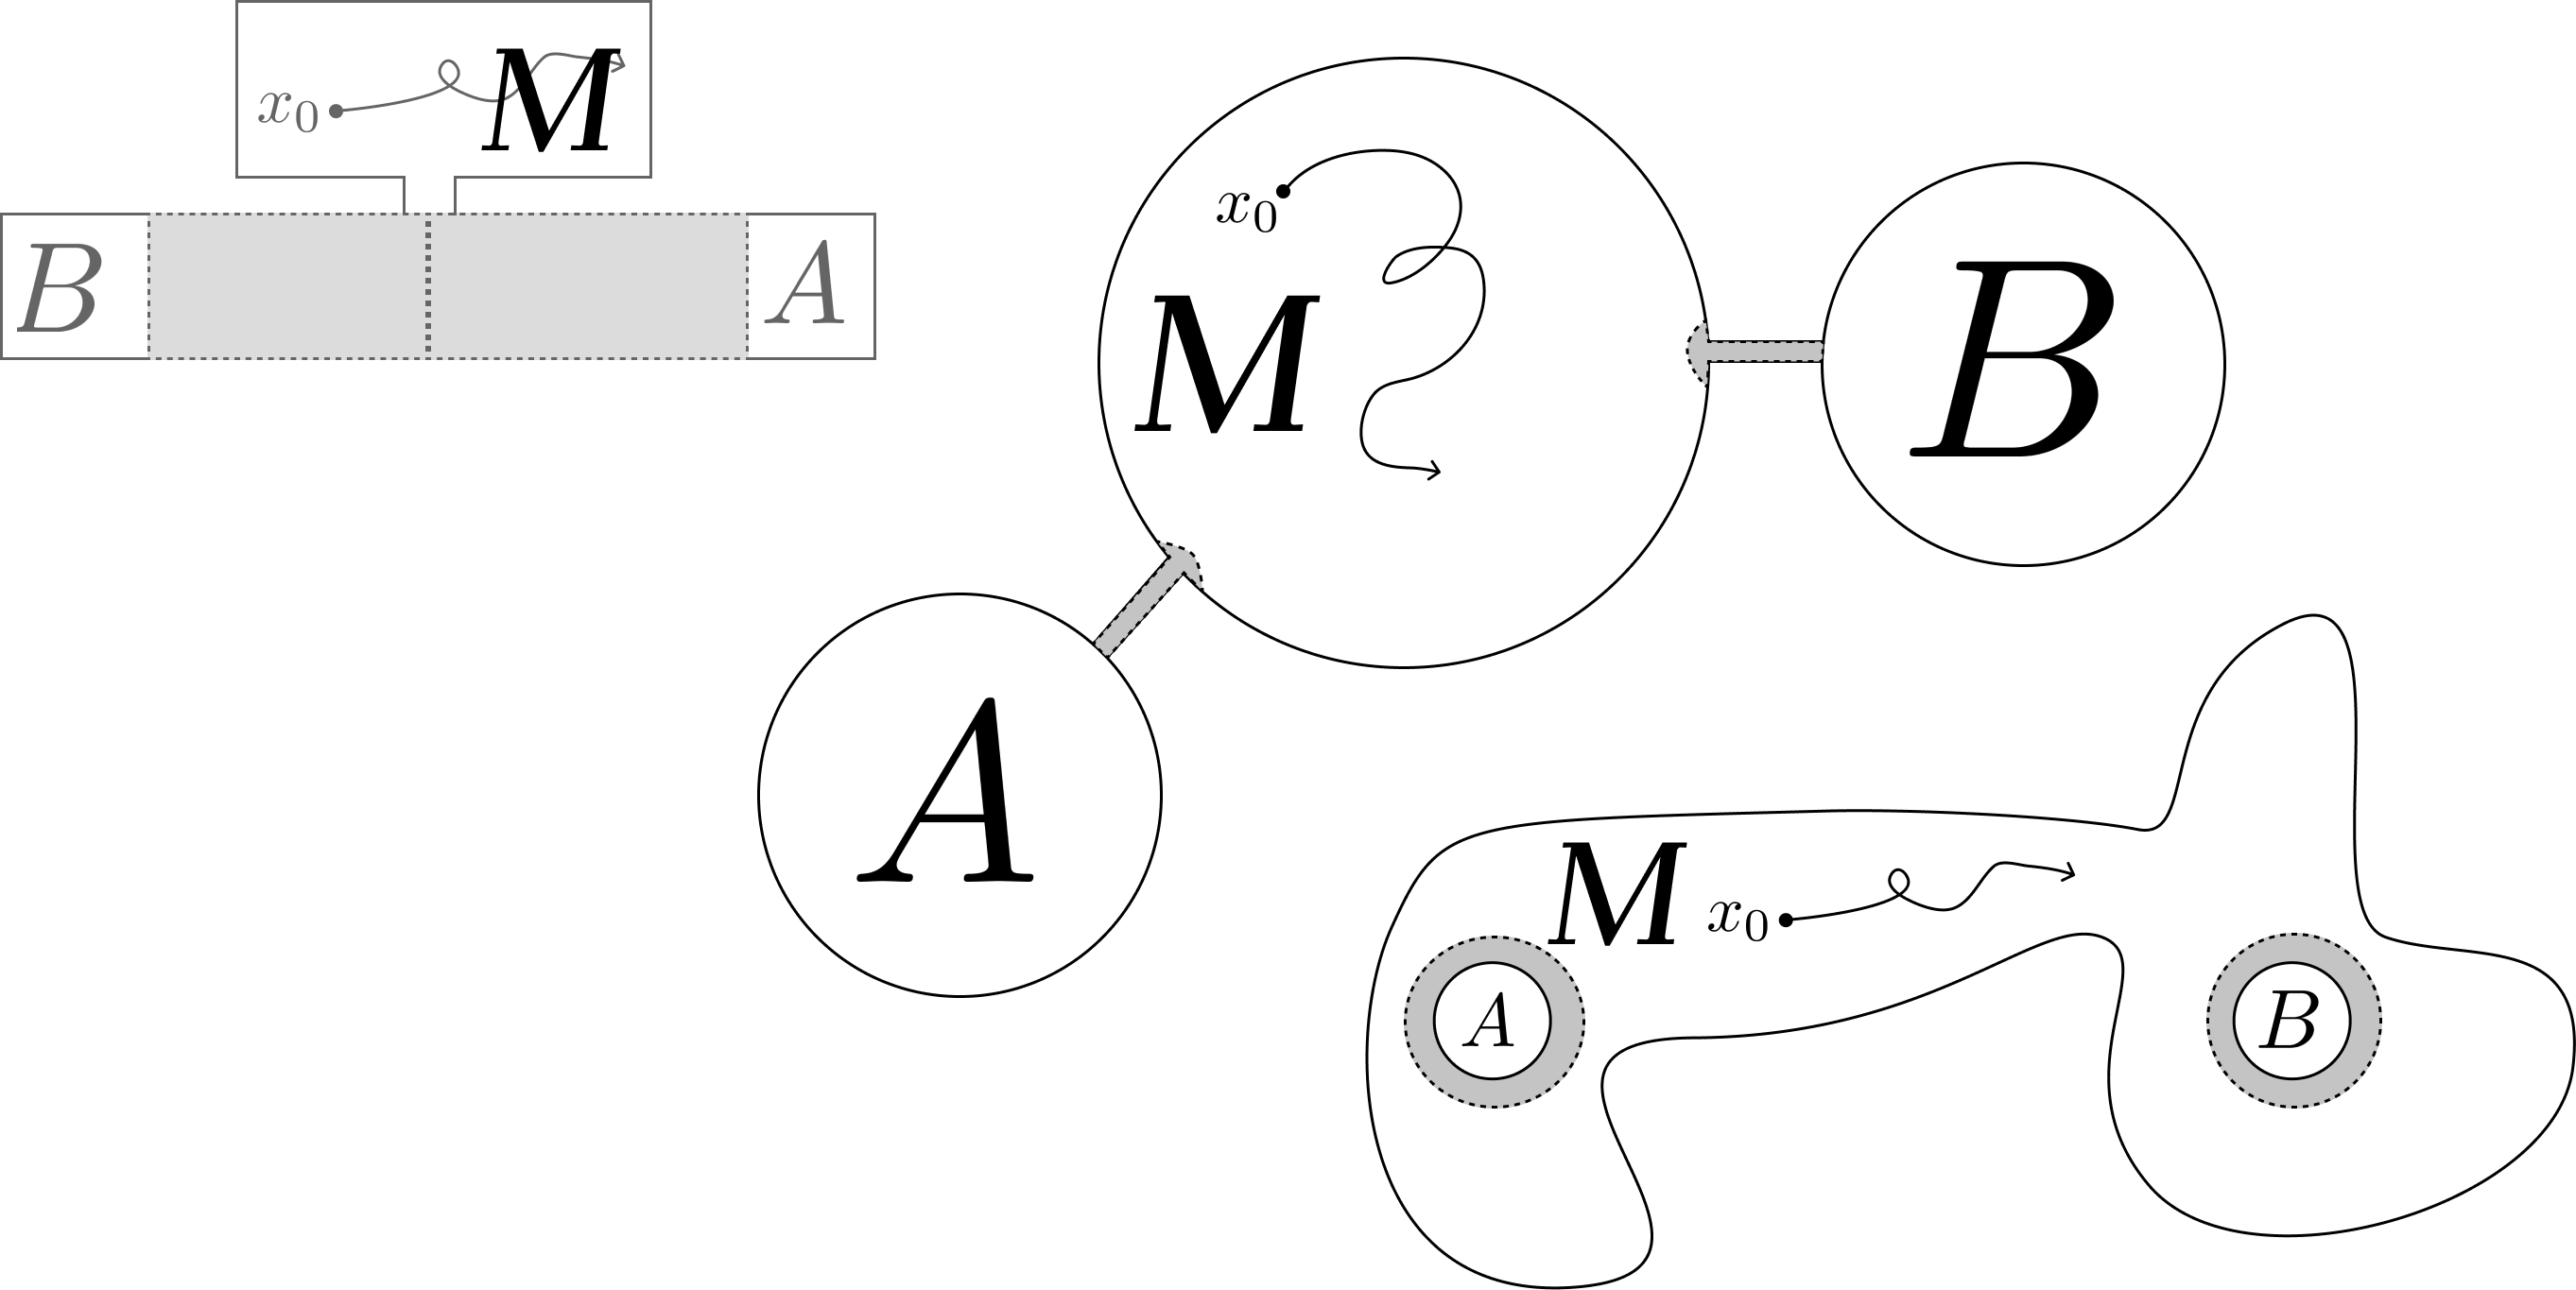
\includegraphics[width=0.8\textwidth]{bigpicture.png}
    \caption{\footnotesize\linespread{1.}\selectfont{} {\bf First passage capacities allow efficient computation of hitting probabilities.} We consider a reversible stochastic differential equation in an $n$-dimensional state-space.  Let us say we initialize the diffusion at some configuration $x_0$ inside the set $M$; what is the probability it will reach region $A$ first before $B$?  We assume that the hitting probability is nearly the same for every initial condition $x_0 \in M$ -- it must differ by at most $\varepsilon$ among all such initial conditions.  Theorem \ref{thm:main_thm} then shows that the hitting probability can then be approximated to within $\varepsilon + \sqrt{\varepsilon/2}$ using only ``first passage capacities.'' These capacities can be computed using only simulations that take place outside of $M$.  Above we sketch several examples where the condition can hold.  In each case, the first passage capacities can be computed efficiently using local simulations performed in the gray areas.}
\label{fig:ToyModel}
\end{figure}

In the following section (\S\ref{sec:Preliminaries}, ``Preliminaries'') we will introduce notation, define our diffusion, define first passage hitting probabilities, define our main assumption, and finally define the first-passage capacities that are at the heart of this approach.  In \S\ref{sec:MainResults} we show that these capacities can be used to accurately estimate first-passage probabilities as long as our assumption holds; we also give examples where this condition is guaranteed.  In \S\ref{sec:Estimation}, we develop an algorithm to compute the first passage capacities.   In \S\ref{sec:Experiments} we investigate the speed and accuracy of the capacity-based approach, using computational experiments on various diffusions.

\section{Preliminaries}
\label{sec:Preliminaries}

The results in this paper are about diffusion processes $X$ confined to an open bounded set $\Omega \subset \mathbb{R}^n$ with reflecting smooth boundary $\partial\Omega$ for $n\geq 3$.  We assume $X$ is driven by an $n$-dimensional standard Brownian motion $W$, i.e.
\begin{equation}\label{equ:general_sde}\mathrm{d} X_t = b (X_t) \mathrm{d} t + \sigma (X_t) \mathrm{d} W_t \end{equation}
where $b: \Omega \rightarrow \mathbbm{R}^n$ and $\sigma :
\Omega \rightarrow \mathbbm{R}^{n \times n}$ are continuously differentiable vector-valued and matrix-valued functions.  We further assume that $a(x)=\sigma(x)\sigma(x)^T$ is uniformly elliptic on $\Omega$, i.e. the smallest eigenvalues of $a$ are bounded away from zero.  Let $\bar \Omega$ denote the closure of $\Omega$ (and in general let $\bar S$ denote the closure of any set $S\subset \bar \Omega$).  For the precise definition of the reflected process, we adopt the framework developed by Lions and Sznitman\cite{lions1984stochastic}: Let $\normal=\normal(x)$ denote the outward normal of $\partial \Omega$ and $\nu:\ \partial \Omega \rightarrow \mathbb{R}^n$ a smooth vector field satisfying $\normal^T\nu\geq c>0$, and assume that $x_0 \in \Omega$.  Then there is a unique pathwise continuous
and $W$-adapted strong Markov process $X_t\in\bar\Omega$, and (random) measure $L$, such that
\begin{gather}\label{eq:SDER}
X_t = x_0 + \int_0^t b(X_s)ds + \int_0^t \sigma(X_s)dW_s - \int_0^t \nu(X_s) L(ds)
\end{gather}
and $L(\{t:\ X_t \notin \partial \Omega\})=0$.
For convenience, we will refer to $X$ by simply saying ``the reflected diffusion process (\ref{equ:general_sde}).'' We further assume that $X$ is a reversible process, with equilibrium distribution given by
\[
\rho(x)\doteq \frac{1}{Z}e^{-U(x)}\ \ \
Z=\int_{x\in\Omega}e^{-U(x)}dx
\]
where $U:\bar \Omega \rightarrow \mathbb{R}$ is continuously differentiable.  As shown by Chen \cite{chen1993reflecting}, to ensure that $X$ is reversible it is sufficient that
\begin{align}
\begin{split}
b_i(x)&=\frac{1}{2} \sum_j \partial a_{ij}(x)/\partial x_j - \frac{1}{2}\sum_j a_{ij}(x) \partial U(x)/\partial x_j
\label{eqn:reversibility} \\
\nu(x)&= a(x) \normal(x)
\end{split}
\end{align}
where $a(x)=\sigma(x)\sigma(x)^T$ is uniformly elliptic.
When the conditions in (\ref{eqn:reversibility}) are in force
we will say that $X$ satisfies the reversibility conditions relative to $U$.  We assume these conditions throughout the paper.

The main goal of this paper is to estimate first passage hitting probabilities for $X$.  We here give a formal definition for these hitting probabilities:

\begin{definition}(First passage hitting probabilities).  Fix two disjoint sets $A,B\subset \Omega$.  The first-passage hitting probability function $h_{A,B}(x)$ indicates the probability that the process $X$ visits $A$ before $B$ if it is initialized at $X_0=x$.  Formally,
\[ h_{A, B}(x) \triangleq \mathbb{P}(X_{\tau_{A\cup B}}\in A|X_0=x)\]
where $\tau_{A\cup B}$ indicates the first passage time to $A\cup B$, i.e.\ $\tau_{A\cup B} \triangleq \inf \{ t \geqslant 0 : X_t \in A \cup B \}$.  Throughout this paper we will use $\tau_S$ to denote the first passage time to a set $S$ and $h_{S,S'}$ to denote the hitting probability function for targets $S,S'$.
\end{definition}

As discussed in the introduction, these hitting probabilities are much easier to estimate if the process forgets its initial condition to such an extent that the hitting probabilities are nearly constant for any initial condition inside a set $M$.  Here we give a formal definition for this property:
\begin{definition}(The $\varepsilon$-flatness condition)  A hitting probability function $h_{A,B}(x)$ is said to be
``$\varepsilon$-flat relative to $M$'' whenever
\[
\sup_{x, y \in M} |h_{A,B}(x) - h_{A,B}(y)| < \varepsilon
\]
\end{definition}
As we shall see in Theorem \ref{thm:main_thm}, this condition is exactly what we need to show that the hitting probabilities within $M$ can be well-approximated using ``first-passage capacities.''  These capacities are the last piece we must define:

\begin{definition}(Capacity)
Let $S \subset \tilde{S} \subset \Omega$ be open sets and let $X$ be a diffusion governed by the SDE in Equation (\ref{eq:SDER}) and satisfying the reversibility conditions in Equation (\ref{eqn:reversibility}).  The first-passage capacity $\ensuremath{\operatorname{cap}} (S, \tilde{S})$ for $X$ is defined as
%
\[ \ensuremath{\operatorname{cap}} (S, \tilde{S}) \triangleq \int_{\tilde S \backslash S}
||\sigma(x) \nabla h_{S, \tilde{S}^c}(x)||^2 e^{- U(x)} \mathrm{d} x \]
%
\end{definition}

We refer the reader to Appendix \ref{sec:three_perspectives} for more details on capacity and the related concept of Dirichlet form.  Note that there are several related definitions of ``capacity'' in the probabilistic potential theory literature, all slightly different.  For example, the Harmonic capacity arises by taking the above definition in the special case when the diffusion is a simple Brownian motion.  The definition used here most closely follows the work of Bovier \cite{Bovier2016-ez,Bovier2004-wj}.  Throughout this work, the term is used only in the sense of the above definition.

\section{Main theoretical results}
\label{sec:MainResults}

Our main theorem shows that the first-passage capacities give accurate approximations of the hitting probabilities when the hitting probabilities are themselves $\varepsilon$-flat in a region outside a neighborhood of the targets.

\begin{theorem}\label{thm:main_thm}
Let $A\subset \tilde A,B\subset \tilde B$ be open sets and assume that  $h_{A,B}(x)$ is $\varepsilon$-flat relative to
$\Omega \backslash (\tilde A \cup \tilde B)$.
Then the first-passage probabilities are well-approximated by the first-passage capacities:
\[ \sup_{x \notin \tilde A,\tilde B} \left| h_{A,B} (x) - \frac{\capac{A}{\tilde A}}{\capac{A}{\tilde A}+\capac{B}{\tilde B}} \right| \leqslant \varepsilon + \sqrt{\varepsilon/2} \]
\end{theorem}

We defer the proof to Appendix \ref{sec:proof_thm}.  Note that the generalization to multiple targets is straightforward due to the additive property of capacities (Proposition \ref{prop:capacity} in Appendix \ref{sec:three_perspectives}).  In general, the hitting probability is approximately proportional to the corresponding capacity.

When might the $\varepsilon$-flatness condition hold?  In the introduction, we gave an intuitive explanation for when this might be expected to happen, namely whenever the diffusion forgets its initial condition before it hits the targets.  To prove the $\varepsilon$-flatness condition for a particular problem, one must make this idea rigorous.  To offer the reader a flavor for how this may be done, we offer the following examples:

\begin{theorem}\label{thm:epsilon_flat} (Examples of $\varepsilon$-flatness).   Let $\bb{x,r} = \{y:\ \Vert x-y \Vert < r\}$ denote the ball of radius $r$ centered at $x$.  Let us say that a diffusion governed by Equation (\ref{eq:pde}) ``behaves like Brownian motion'' on a set if $\sigma(x)=I$ and $\nabla U(x)=0$ for every $x$ in that set.  
\begin{enumerate}
    \item Fix $r,\varepsilon>0$.  We can then find $\delta>0$ with the following property.  For any bounded convex set $\Omega$ with diameter less than or equal to 1, any $x_A,x_B \in \Omega$, any reversible stationary diffusion trapped inside $\Omega$ and behaving like Brownian motion for all $x\notin \bb{x_A, \delta} \cup \bb{x_B, \delta}$, and any $A\subset \bb{x_A, \delta}, B \subset \bb{x_B, \delta}$, we have that $h_{A,B}$ is $\varepsilon$-flat on $\Omega \backslash \bb{x_A, r} \cup \subset \bb{x_B, r}$.

    \item Fix $r,\varepsilon>0$ and $r'<r$.  We can then find $n$ with the following property.  For any convex set $\Omega \in \mathbb{R}^n$ with diameter less than or equal to 1, any $x_A,x_B$ such that $\bb{x_A, r},\bb{x_B, r} \subset \Omega$, any reversible stationary diffusion trapped inside $\Omega$ and behaving like Brownian motion for all $x\notin \bb{x_A, r'} \cup \bb{x_B, r'}$, and any $A\subset \bb{x_A, r'}, B \subset \bb{x_B, r'}$, we have that $h_{A,B}$ is $\varepsilon$-flat on $\Omega \backslash \bb{x_A, r} \cup \subset \bb{x_B, r}$.
\end{enumerate}
\end{theorem}

A proof can be found in Appendix \ref{sec:proof_epsilon_flat}.  The first example shows how hitting probabilities become flat as the targets become small.  The second example notes that even if we fix the radius of the targets, the hitting probabilities becomes flat if the ambient dimension $n$ is high.  In both cases, the results are proved by showing that the rate of mixing inside $M$ is fast and it generally takes a long time to leave $M$.

%      _          _ _                _   _               _ 
%  ___| |__   ___| | |_ __ ___   ___| |_| |__   ___   __| |
% / __| '_ \ / _ \ | | '_ ` _ \ / _ \ __| '_ \ / _ \ / _` |
% \__ \ | | |  __/ | | | | | | |  __/ |_| | | | (_) | (_| |
% |___/_| |_|\___|_|_|_| |_| |_|\___|\__|_| |_|\___/ \__,_|
                                                         


\section{Capacity Estimation via the Shell Method}
\label{sec:Estimation}
To make use of Theorem \ref{thm:main_thm} in practice, we must be able to compute capacities.  The calculation is local, in that $\capac{A}{\tilde{A}}$ is an integral on $\tA\backslash A$. We will propose here a Monte Carlo approach to evaluating the integral, using a combination of analytic reductions and a short location simulations.

We begin by using an alternative formulation of the capacity:

\begin{proposition}
\label{prop:flux}
For any regions $G$ and $\tilde{G}$ having smooth boundaries and such that $A\subset G \subset \tilde G \subset \tilde A$, $\capac{A}{\tA}$ can be expressed as a flux leaving $\tilde G \backslash G$:
\begin{equation}
\label{eqn:GIntegral}
\ensuremath{\operatorname{cap}} (A, \tilde{A}) = \int_{\partial (\tilde G \backslash G)}  h_{A, \tilde{A}^c} (x)   \normal(x)^T a (x) \nabla h_{G, \tilde{G}^c} (x)e^{- U (x)} \hausdorffmeasure
\end{equation}
where $a(x)=\sigma(x)\sigma(x)^T$ is the diffusion matrix, $\hausdorffmeasure$ is the $(n-1)$-dimensional Hausdorff measure, and $\normal$ represents the outward-facing (relative to the set $\tilde G \backslash G$) normal vector on $\partial (\tilde G \backslash G)$.
\end{proposition}
\noindent This result is already known, though we could not find it written down in exactly the form we need.  A formal proof is in Appendix \ref{sec:proof_proposition}.

There is a great deal of freedom in choosing $G$ and $\tilde G$; the idea is to choose them so as to make the surface integrals as simple as possible.  Each of these surface integrals can be viewed as an expectation.  Let $\hausdorffmeasure$ denote the $n-1$-dimensional Hausdorff measure.  We can define a probability measure on
$\partial G$ by
\[
\PMeasure\doteq\frac{1}{Z}e^{-U(x)}\hausdorffmeasure
\text{   where   }
Z= \int_{\partial G} e^{-U(x)}\hausdorffmeasure
\]
We can define $\tPMeasure$
and $\tilde{Z}$ analogously, on $\partial\tilde{G}$ rather than $\partial G$.
Then
\begin{align}
\capac{A}{\tilde A} & = \int_{\partial\tilde{G}} h_{A, \tilde{A}^c}    \normal^T a  \nabla h_{G, \tilde{G}^c} e^{- U } \hausdorffmeasure
-\int_{\partial G} h_{A, \tilde{A}^c}    \normal^T a  \nabla h_{G, \tilde{G}^c} e^{- U } \hausdorffmeasure
\nonumber \\
&=\tilde Z
\int_{\partial\tilde{G}} h_{A, \tilde{A}^c}    \normal^T a  \nabla h_{G, \tilde{G}^c} \tPMeasure
-Z
\int_{\partial G} h_{A, \tilde{A}^c}    \normal^T a
\nabla h_{G,\tilde{G}^c} \PMeasure
\label{eqn:PMeasureInt}
\end{align}
where, in these integrals, the normal, $\normal$, points outward from both $G$ and $\tilde G$.
Let $y_1,y_2,\dots,y_m\sim \text{iid}\ \PMeasure$, so that
\begin{align*}
\frac{1}{m}\sum_{i=1}^m
h_{A, \tilde{A}^c}(y_i) \normal^T(y_i) a(y_i)  \nabla h_{G,\tilde{G}^c}(y_i) & \stackrel{m\to\infty}{\longrightarrow}
 \int_{\partial G} h_{A, \tilde{A}^c}    \normal^T a
\nabla h_{G,\tilde{G}^c} \PMeasure \\
\text{and}\ \ \ \ \ \ \frac{1}{m}\sum_{i=1}^m e^{U(y_i)}
& \stackrel{m\to\infty}{\longrightarrow} \int_{\partial G} e^U
\PMeasure = \frac{|\partial G|}{Z}
\end{align*}
where $|\partial G|$ is the surface area of $G$. Putting these together, we get the large $n$ approximation
\[
Z
\int_{\partial G} h_{A, \tilde{A}^c}    \normal^T a
\nabla h_{G,\tilde{G}^c} \PMeasure
\approx
|\partial G|
\frac{\sum_{i=1}^m
h_{A, \tilde{A}^c}(y_i) \normal^T(y_i) a(y_i)  \nabla h_{G,\tilde{G}^c}(y_i)}
{\sum_{i=1}^m e^{U(y_i)}}
\]
If we now extend all of this to $\partial\tilde{G}$, with
$\tilde{y}_1,\tilde{y}_2,\dots,\tilde{y}_n\sim \text{iid}\ \tPMeasure$, and put the approximations into
(\ref{eqn:PMeasureInt}), then for large $n$ and $m$
\begin{align}
\capac{A}{\tilde A} & \approx
|\partial\tilde{G}|
\frac{\sum_{i=1}^n
h_{A, \tilde{A}^c}(\tilde{y}_i) \normal^T(\tilde{y}_i) a(\tilde{y}_i)  \nabla h_{G,\tilde{G}^c}(\tilde{y}_i)}
{\sum_{i=1}^n e^{U(\tilde{y}_i)}}
\label{eqn:approximate_capacity}\\
& -|\partial G|
\frac{\sum_{i=1}^m
h_{A, \tilde{A}^c}(y_i) \normal^T(y_i) a(y_i)  \nabla h_{G,\tilde{G}^c}(y_i)}
{\sum_{i=1}^m e^{U(y_i)}}
\nonumber
\end{align}

In summary: we can use a Monte-Carlo technique to compute the capacity as long as we can (i) sample from $\PMeasure$ and $\tPMeasure$; (ii) compute the surface areas $|\partial G|$ and
$|\partial\tilde{G}|$; (iii)
compute the first-passage probability $h_{A, \tilde{A}^c}$; and (iv) compute the gradient
$\nabla h_{G, \tilde{G}^c}$.  
We can often make tasks (i) and (ii) straightforward by a judicious choice of $G,\tilde G$.  However, tasks (iii) and (iv) are more difficult.  

Thus, to compute the capacity using this approach, the most difficult challenge is to compute the first-passage probabilities along $G,\tilde G$.  Broadly speaking there are two approaches for this kind of problem.  First-passage probabilities satisfy an elliptic PDE related to the infinitesimal generator -- see Appendix \ref{sec:three_perspectives}, Equation (\ref{eq:pde}) -- and we could therefore choose from a selection of numerical solvers. Here, in a different direction, we exploit the connection between first-passage probabilities and the underlying random walk in order to develop Monte Carlo tools suitable for estimating both $h_{A, \tilde{A}^c}$ and $\nabla h_{G, \tilde{G}^c}$ on the surfaces
$\partial G$ and $\partial\tilde{G}$. These tools are based on
what we will call the ``shell method,'' which we describe briefly in the following paragraphs and in full detail in Appendix \ref{sec:shell_method}.

Generically, given two simply-connected regions $R$ and $\tilde{R}$, with $R\subset \tilde{R}$, and a set $S$ such that
$R\subset S  \subset\tilde{R}$, we seek an approximation to
the function $h_{R,\tilde{R}^c}$ on the surface $\partial S$. In principle, we could begin with a fine-grained partitioning of $\partial S$ into simply-connected ``cells,'' and for each cell simulate the diffusion many times, recording whether or not the path first exits $\partial (\tilde{R}\backslash R)$ at $\partial R$. The fraction of paths that first exit at $\partial R$ constitutes an estimate of
$h_{R,\tilde{R}^c}(x)$ for any $x$ in the current cell. But this is wasteful and likely infeasible in all but the simplest of settings. Much of the waste stems from the fact that the ensemble of all paths generated from all cells will likely include many near collisions of paths scattered throughout $\partial (\tilde{R}\backslash R)$. An alternative, divide-and-conquer  approach, is to introduce multiple sets, $S_0,S_1,\ldots,S_n$ such that
\begin{equation*}
R=S_0 \subset \cdots \subset S_{m-1}\subset S_m = S \subset S_{m+1} \subset \cdots \subset S_n = \tilde{R}
\end{equation*}
and use sample paths from $X$, {\em locally}, to estimate the transition probability matrices from each cell within each ``shell'' $\partial S_k$ to each cell of its neighboring shells, $\partial S_{k-1}$ and $\partial S_{k+1}$. Equipped with these transition matrices, the first-passage probability for a given $x\in S$ is computed algebraically, without further approximation.

$S$ must have been chosen not only to satisfy $R\subset S  \subset\tilde{R}$ but also in such a way as to make it feasible to sample from $\partial S$ under the probability measure
$\frac{1}{Z}e^{-U}\hausdorffmeasure$. After that, $S_k\ k=1,\ldots,n-1$ are chosen so that the shells nest and are in close proximity; the hitting times starting from a sample in $\partial
 S_k$ and ending at $\partial S_{k-1} \cup \partial S_{k+1}$ must be short enough to encourage many repeated runs. The output is a set of samples,
 $z_1,\ldots,z_N \sim \frac{1}{Z}e^{-U}\hausdorffmeasure$ on $\partial S$ together with the approximate value of $h_{R,\tilde{R}^c}(x)$ at each sample $x=z_i$. (In fact, though the main purpose is to estimate $h_{R,\tilde{R}^c}$ on
 $\partial S$, a byproduct is a sample from $\frac{1}{Z}e^{-U}\hausdorffmeasure$ on all of the shells $\partial S_k$, along with an estimate of $h_{R,\tilde{R}^c}$ at every sample.)
With the choice of $A$ for $R$ and $\tilde A$ for $\tilde R$, the algorithm becomes directly applicable to the estimation of $h_{A, \tilde{A}^c}$ on $\partial G$ and $\partial\tilde{G}$, taking $S=G$ in the former case and $S=\tilde{G}$ in the latter.

The shell method is closely related to milestoning\cite{West2007-cn, Bello-Rivas2015-ld, Aristoff2016-gc} and Markov state models\cite{Pande2010-yi, Chodera2014-bh, Husic2018-xp}, though more tailored to the problem at hand. In particular, our interest here is in computing the first-passage probabilities rather than in approximating the underlying process. Also, the discretizations of the shells are {\em adaptive}, in that they are based on clusters that are derived from an ensemble of samples, as opposed to being crafted for a particular landscape.  See Appendix \ref{sec:shell_method}.

As for the required gradients, these are generally harder to estimate. Nevertheless, for the particular gradient $\nabla h_{G, \tilde{G}^c}$, the problem is substantially mitigated by noting that we are only interested in its evaluation on $\partial G$ and $\partial\tilde G$, each of which is a level set of
$h_{G, \tilde{G}^c}$ ($h_{G, \tilde{G}^c}=1$ on $G$ and 0 on $\tilde G$). Consequently, on each surface the gradient is in the normal direction and we need only estimate its magnitude. And for this purpose it is enough to know the values of $h_{G, \tilde{G}^c}$ on a surface close to $G$ and interior to $\tilde{G}\backslash G$ (for estimating $\nabla h_{G, \tilde{G}^c}$ on $G$) and on another surface
close to $\tilde{G}$ and also interior to $\tilde{G}\backslash G$ (for estimating $\nabla h_{G, \tilde{G}^c}$ on $\tilde G$). Two such surfaces would be $\partial S_1$ and $\partial S_{n-1}$, were we to apply the shell method with $R=G$ and $\tilde{R}=\tilde{G}$,
since, as already noted, a byproduct of the method is an estimate of
$h_{R,\tilde{R}^c}$ on all of the shells. Alternatively, in the interest of better accuracy, the method could be run twice, once with $S=S_1$, a well-chosen outer approximation of $G$, and then again with
$S=S_{n-1}$, a well-chosen inner approximation of $\tilde G$.

%%%%%%%%%%%%%%%%%%%%%%%%%%%%%%%%%%%
%%%%%%%%%%%%%%%%%%%%%%%%%%%%%%%%%%%
%%%%%%%%%%%%%%%%%%%%%%%%%%%%%%%%%%%
%%%%%%%%%%%%%%%%%%%%%%%%%%%%%%%%%%%

%                                  _           _                       _ _       
%  _ __  _   _ _ __ ___   ___ _ __(_) ___ __ _| |  _ __ ___  ___ _   _| | |_ ___ 
% | '_ \| | | | '_ ` _ \ / _ \ '__| |/ __/ _` | | | '__/ _ \/ __| | | | | __/ __|
% | | | | |_| | | | | | |  __/ |  | | (_| (_| | | | | |  __/\__ \ |_| | | |_\__ \
% |_| |_|\__,_|_| |_| |_|\___|_|  |_|\___\__,_|_| |_|  \___||___/\__,_|_|\__|___/
                                                                               


\section{Numerical Experiments\footnote{All the experimental results can be reproduced or easily modified from open-source code, which can found, along with detailed instructions, at \url{https://github.com/StannisZhou/entropic_barrier}.}}\label{sec:Experiments}
We use numerical experiments to test the practical relevance of our theoretical results and capacity-estimation algorithm.  There several questions we would like to address empirically:

\begin{itemize}
    \item When are first-passage hitting probability functions flat?  Recall that the first-passage capacity method is only guaranteed to be accurate when this flatness condition holds.  Theorem \ref{thm:epsilon_flat} gives conditions for the first-passage hitting probability function to become flat in the asymptotic limit as the targets become small.  How quickly do these asymptotic limits begin to apply?  What kinds of diffusions actually satisfy $\varepsilon$-flatness condition with $\varepsilon \ll 1$?
	\item Is Theorem \ref{thm:main_thm} loose or tight?  This Theorem shows that the first-passing hitting probabilities can be well-approximated by first-passage capacities whenever the first-passage hitting probability function is $\varepsilon$-flat.  Specifically, the theory shows that capacity-based estimates lie within $\theepsrate$ of the truth.  Is this bound is tight or loose?
	\item Is the shell-method accurate and fast?  In Section \ref{sec:Estimation} we propose a new algorithm for estimating the capacity.  What is the speed and accuracy of this algorithm?
\end{itemize}

To test these questions we look at problems of the following form.  In every case the configuration space,
$\Omega$, is the unit ball in $\mathbb{R}^5$.  In other words, 
$\Omega = \bb{0,1}$, where $\bb{x, r} \triangleq \{ y : || y - x || < r \}$. A diffusion is confined to $\Omega$ by a reflecting boundary at $\partial\Omega$, and within $\Omega$ the dynamics are assumed given by the first-order (high-viscosity) Langevin equation,
\begin{equation}
\label{equ:toy_sde}
\mathrm{d} X_t = - \nabla U (X_t) \mathrm{d} t + \mathrm{d} W_t
\end{equation}
where $W_t$ is an $n$-dimensional Brownian motion and
$U$ is a potential energy. There are only two targets,
\begin{align*}
A &\triangleq \bb {x_A, r_A}\\
B &\triangleq \bb {x_B, r_B}
\end{align*}
Given an initial condition $X_0\in \Omega \backslash (A\cup B)$, we are interested to know whether the dynamics carry the system into $A$ or $B$ first.  We further assume that $U$ is constant beyond the immediate neighborhoods of $A$ and $B$; letting $\dA=\bb{x_A,r_\dA }$ and $\tA=\bb{x_A,r_\tA }$ such that $r_A<r_\dA<r_\tA$, letting $\dB=\bb{x_B,r_\dB }$ and  $\tB=\bb{x_B,r_\tB}$ such that $r_B<r_\dB<r_\tB$, we assume that $\nabla U(x)=0$ for all $x\in\Omega\backslash (\dA\cup\dB)$.  We will be particularly interested in initial conditions $X_0 \nin \tA \cup \tB$.

We will consider several variations on the setup described above; each variation will gives us a different perspective on the empirical questions we are seeking to answer.  
\subsection{Brownian Diffusion}
\label{sec:B_D}

\begin{figure}
\fbox{\begin{minipage}{\textwidth}
    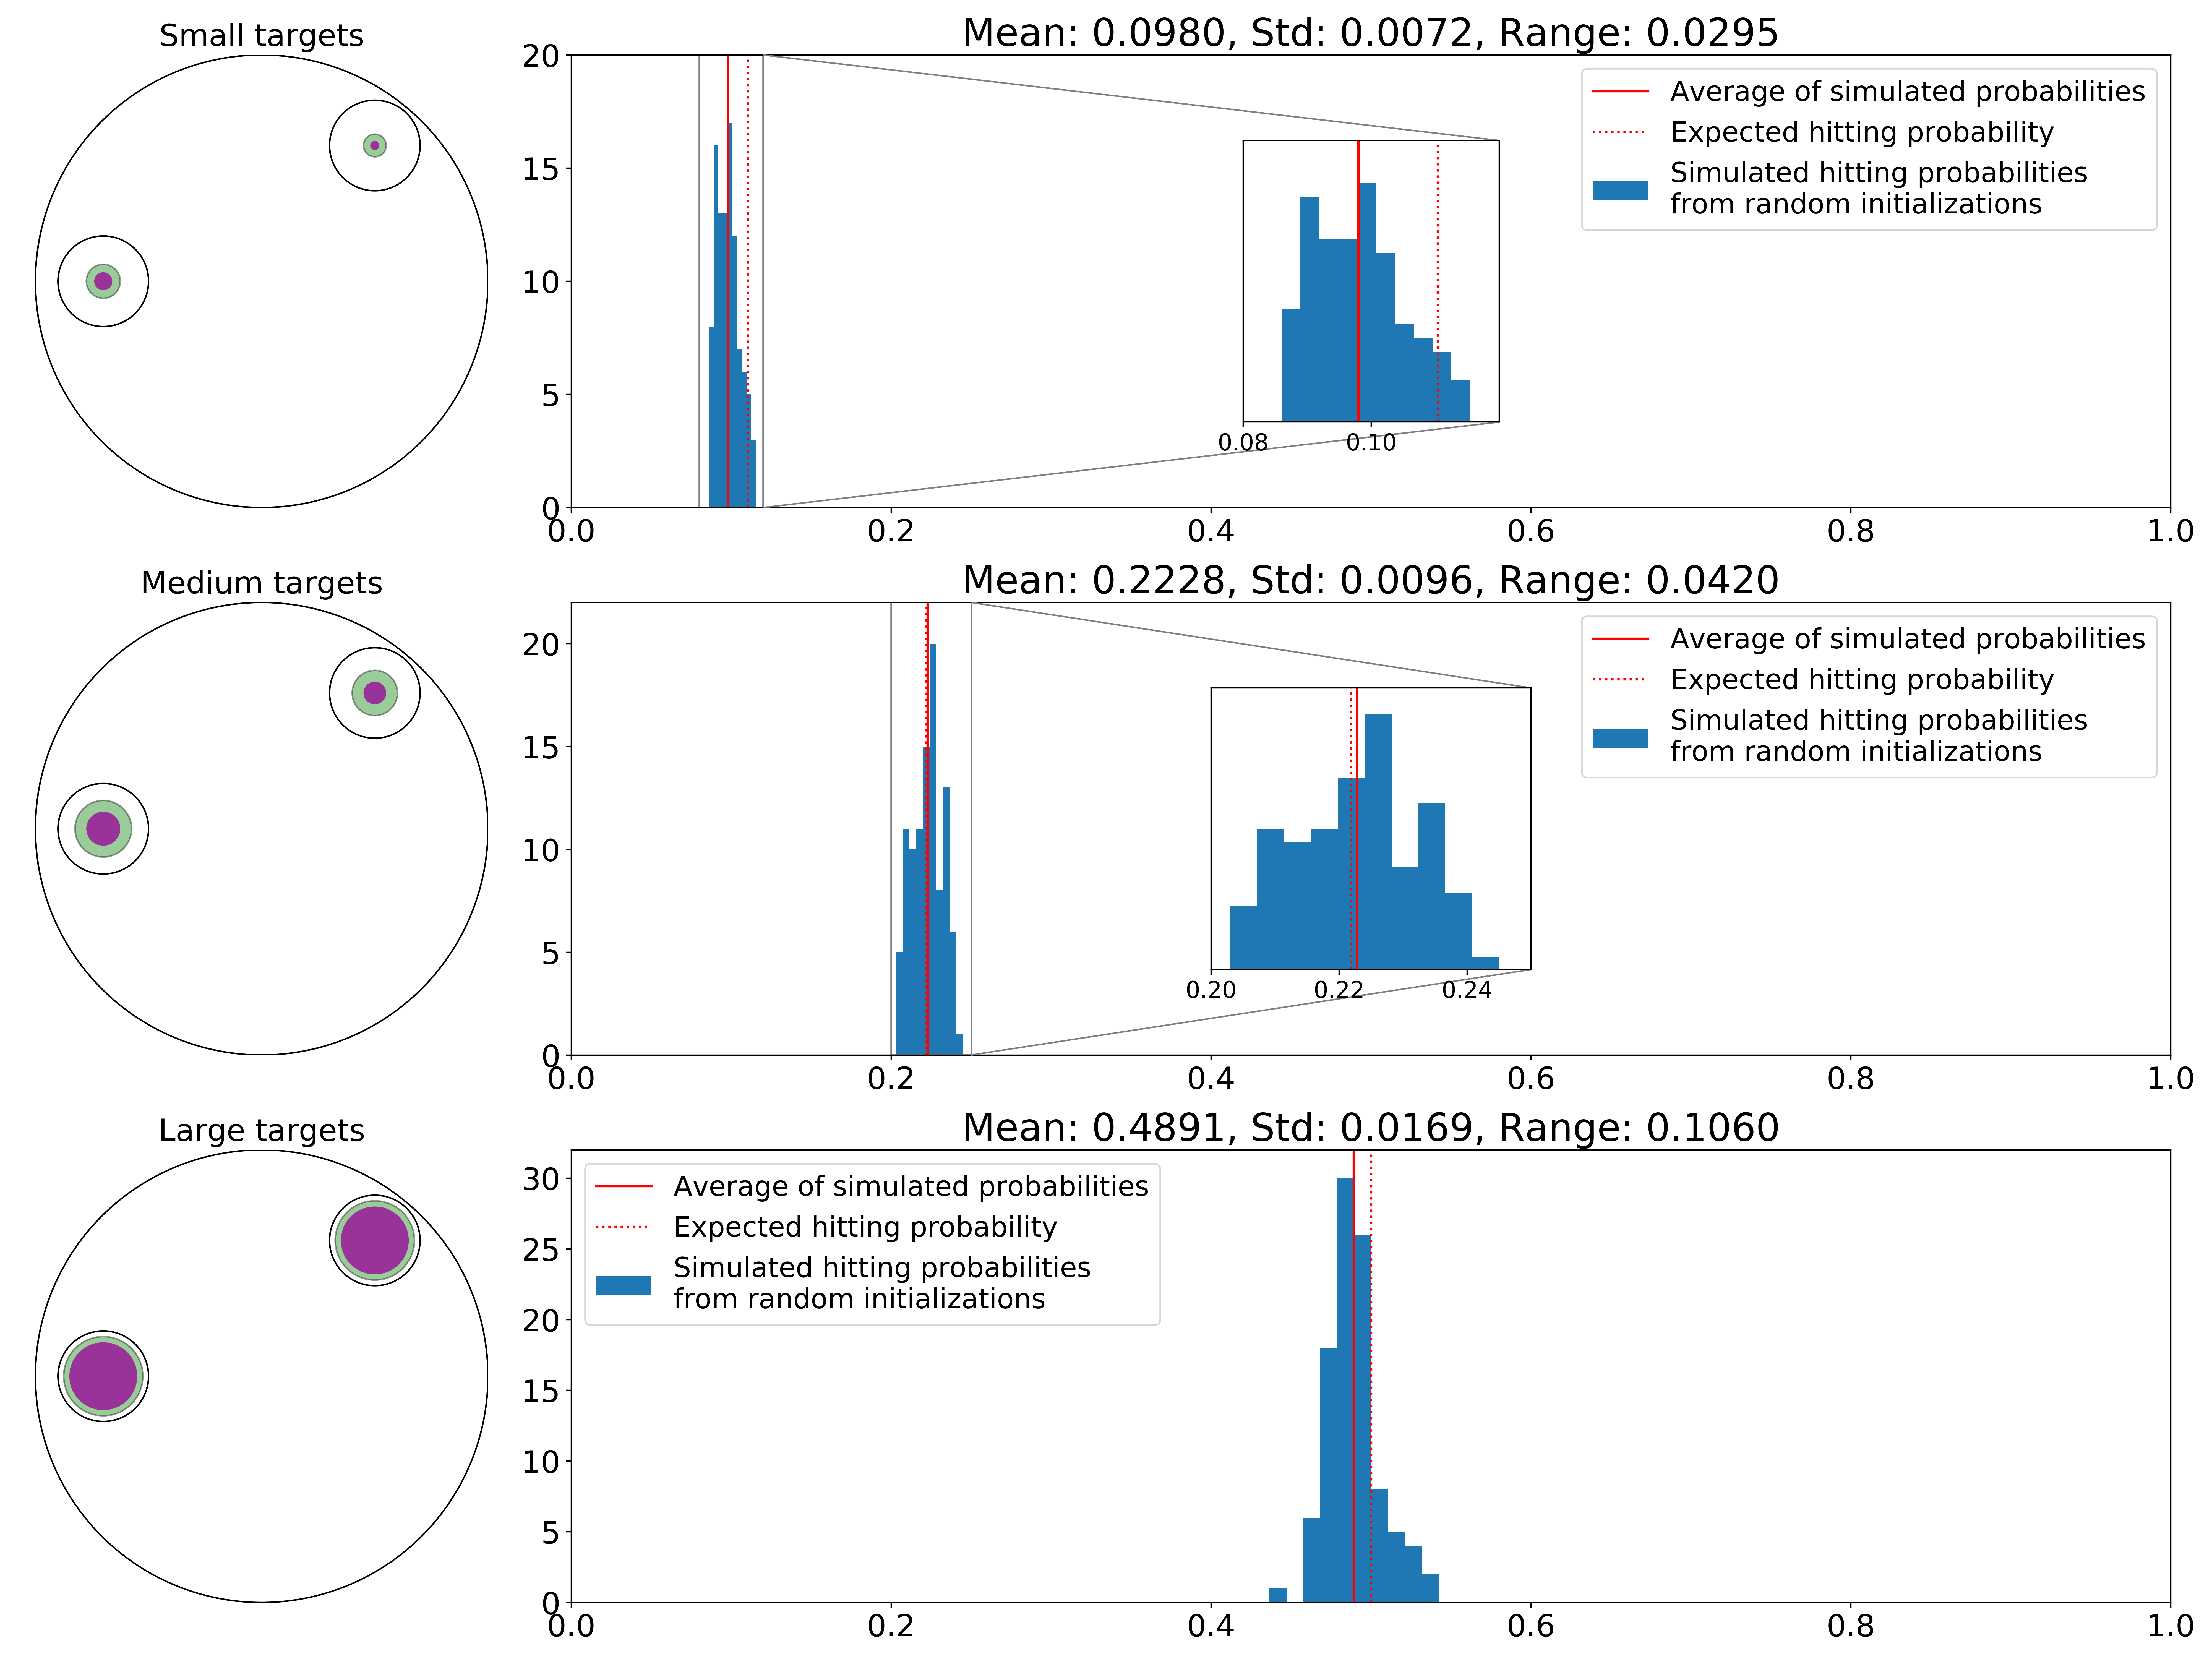
\includegraphics[width=\textwidth]{results_brownian_motion.png}
    \caption{\label{fig:results_brownian_motion}{\bf Local capacities can accurately answer the question ``where will we go next?'' for Brownian motions.}    We consider three different cases (small, medium and large), as illustrated in the left side of the figure.  In each case we have two targets and are interested in the probability that a Brownian motion will target $A$ before target $B$.  We consider 100 random initial locations which are modestly far away from either target; for each initial location, we estimate the probability of hitting target $A$ first.   We plot these 100 hitting probabilities as a histogram.  The histograms reveal that the hitting probabilities fall within a narrow range, especially when the targets are small.  Moreover, we see that the location of this narrow range can be accurately predicted by the capacity-based approximation in Theorem \ref{thm:main_thm} (shown as a dotted red line); this ``Expected hitting probability'' always falls inside the span of the histogram.  We can compare this expected value to an estimate of the hitting probability for a process initialized at a random location, found by averaging over simulations from 200,000 different initial conditions (this is shown as a red line). }
\end{minipage}}
\end{figure}

The first set of experiments tests the capacity-based approach in the simplest possible case: $U(x)=0$.  Using the simple geometry of our setup, a ``walk-on-spheres'' method (cf.\ \cite{bingham1972random}) can efficiently simulate trajectories for this kind of problem.  This allows us to compute something very close to ``ground-truth'' estimates for the hitting probabilities, even though no analytic formula is available and the problem is somewhat high-dimensional.  We can then compare the results of Theorem \ref{thm:main_thm} and \ref{thm:epsilon_flat} against this ground-truth.  

In this set of experiments, we fixed the target centers $x_A=(0.5,0.6,0.0,0,0,0.0), x_B=(-0.7,0.0,0.0,0,0,0.0)$, fixed the radii $r_\tA=r_\tB=0.2$, and varied the radii $r_A,r_B$.  We looked at three different cases: small (where $r_A=0.02, r_B=0.04$), medium (where $r_A=0.05, r_B=0.075$) and large (where $r_A=r_B=0.15$). An illustration of the three different cases and the corresponding results are shown in Figure \ref{fig:results_brownian_motion}.  

For each radius we will be interested in our three main questions.  Does the $\varepsilon$-flatness condition hold?  How well do the first-passage capacities estimate the hitting probabilities?  How accurate and fast is the capacity estimation algorithm?

\subsubsection{Does the $\varepsilon$-flatness condition hold?}
\label{sec:toy_constant}
How much do the hitting probabilities vary as a function of initial condition?  To investigate the relationship between hitting probability and initial condition, we conducted 2,000 diffusion simulations at each of 100 randomly selected initial conditions.  These simulations yielded 100 well-estimated hitting probabilities.  The histograms of these probabilities can be be found in Figure \ref{fig:results_brownian_motion}.  As the targets become smaller, the hitting probability varies less, and these histograms become more peaked.  Based on these histograms we estimate that the flatness of the hitting probability functions are given by:
\begin{itemize}
    \item $\varepsilon\approx 0.0295$ when the targets are small
    \item $\varepsilon\approx 0.0420$ when the targets are medium
    \item $\varepsilon\approx 0.1060$ when the targets are large
\end{itemize}

\subsubsection{Are first-passage probabilities proportional to capacity?}
\label{sec:toy_capacity}
Since the hitting probability functions appear to be fairly flat, Theorem \ref{thm:main_thm} suggests that first-passage capacities should be able to approximate the hitting probabilities according to the formula
\begin{equation}
\label{eqn:capacity_ratio}
h_{A,B}(x) \approx p_A \triangleq \frac{\capac{A}{\tA}}{\capac{A}{\tA}+\capac{B}{\tB}}
\end{equation}
for $x\in M=\mathcal{B}(0, 1) \setminus (\tilde{A} \cup \tilde{B})$.  Theorem \ref{thm:main_thm} shows that this estimate should be accurate to within $\theepsrate$ for a capacity which is $\varepsilon$-flat on the region $M$.  In our case, using the numbers found in the previous section, we calculate that the capacity-based estimates should be accurate to within 15\%, 19\%, and 34\% for small, medium, and large targets respectively.  

In this case we can compute these capacity-based estimates analytically.  The capacities can be computed according to
\begin{equation}
\label{eqn:analytic_capacities}
\capac{A}{\tA}  =
\frac{6\pi^{\frac{5}{2}}}
{\Gamma(\frac{5}{2})(r_A^{-3} - r_\tA^{-3})}  \qquad
\capac{B}{\tB}  =
\frac{6\pi^{\frac{5}{2}}}
{\Gamma(\frac{5}{2})(r_B^{-3} - r_\tB^{-3})}
\end{equation}
The capacity-based estimates are thus given by:
\begin{equation*}
p_A = \frac{\frac{1}{r_A^{-3} - r_{\tilde{A}}^{-3}}}{\frac{1}{r_A^{-3} - r_{\tilde{A}}^{-3}} + \frac{1}{r_B^{-3} - r_{\tilde{B}}^{-3}}}
\end{equation*}
In our case: $p_A \approx 0.1104$ for small targets, $p_A \approx 0.2219$ for medium targets, and $p_A = 0.5$ for large targets.  These are shown as dotted red lines in Figure \ref{fig:results_brownian_motion}.

How accurate are these capacity-based estimates?  In every case, we found the error to be less than $8\varepsilon/9$; this is less than the $\theepsrate$ bound guaranteed by Theorem \ref{thm:main_thm}.   For example, consider the small target case.  For every initial condition we looked at, the true hitting probability lay within 2\% of the capacity-based estimate.  This is much smaller than the 15\% error bound promised by Theorem \ref{thm:main_thm}.  In fact, this error is nearly as low as we could possibly get, given that $\varepsilon \approx 2.3\%$ for small targets.  That is, the true hitting probabilities vary by 2.3\% as we vary the initial condition within $M$.  We are attempting to summarize these different hitting probabilities with a single number: the capacity-based estimate.  To minimize error, the best case would be that the capacity-based estimate was directly in the middle of the variability; this would lead to an error or $\varepsilon/2$.  In fact, we achieve an error of about $8\varepsilon/9$ for the small targets.  Considered as a proportion of the $\varepsilon$ coefficient, the error is even smaller for the the medium- and large-target cases because the estimates lay more directly in the middle of the variability.  

This suggests the possibility that it might be possible to tighten the bound in Theorem \ref{thm:main_thm}.

\subsubsection{Accuracy and speed of the shell method.}
\label{sec:toy_shell}
We here check the accuracy of the capacity estimation algorithm that we call the shell method (cf. \S\ref{sec:Estimation}). For small targets, we find that $\capac{A}{\tA}=0.000632$ and $\capac{B}{\tB}=0.005094$, while shell method estimates them to be $0.000549$ and $0.004699$, respectively. For medium targets, the true capacities are $\capac{A}{\tA}=0.01002626$ and $\capac{B}{\tB}=0.03516428$, while shell method estimates them to be $0.00930769$ and $0.03362453$, respectively. For large targets, the true capacities are $\capac{A}{\tA}=\capac{B}{\tB}=0.4609372$, while shell method estimates them to be $0.45244093 $ and $0.45153703$, respectively.\footnote{With reference to Appendix \ref{sec:shell_method}, the following parameters were used to implement the shell method: $m = 2, n = 4, N_p = 100, N_b = 3, N_s = 1000$, and a time-step of $10^{-7}$.}

Had we used the shell-method to estimate capacities instead of the exact capacities in computing $p_A$ from Equation
(\ref{eqn:capacity_ratio}), we would have obtained different estimates of the first-passage probability: 0.1091 instead of 0.1104 for small targets, 0.2168 instead of 0.2219 for medium targets, and 0.5005 instead of 0.5 for large targets.  Note that these errors are all at least ten times smaller than the $\varepsilon$ coefficients.  As discussed above, $\varepsilon/2$ is the lowest error we could possibly hope to achieve.  Thus the the shell method does not introduce any significant additional error for these problems.

\begin{figure}
\fbox{\begin{minipage}{\textwidth}
    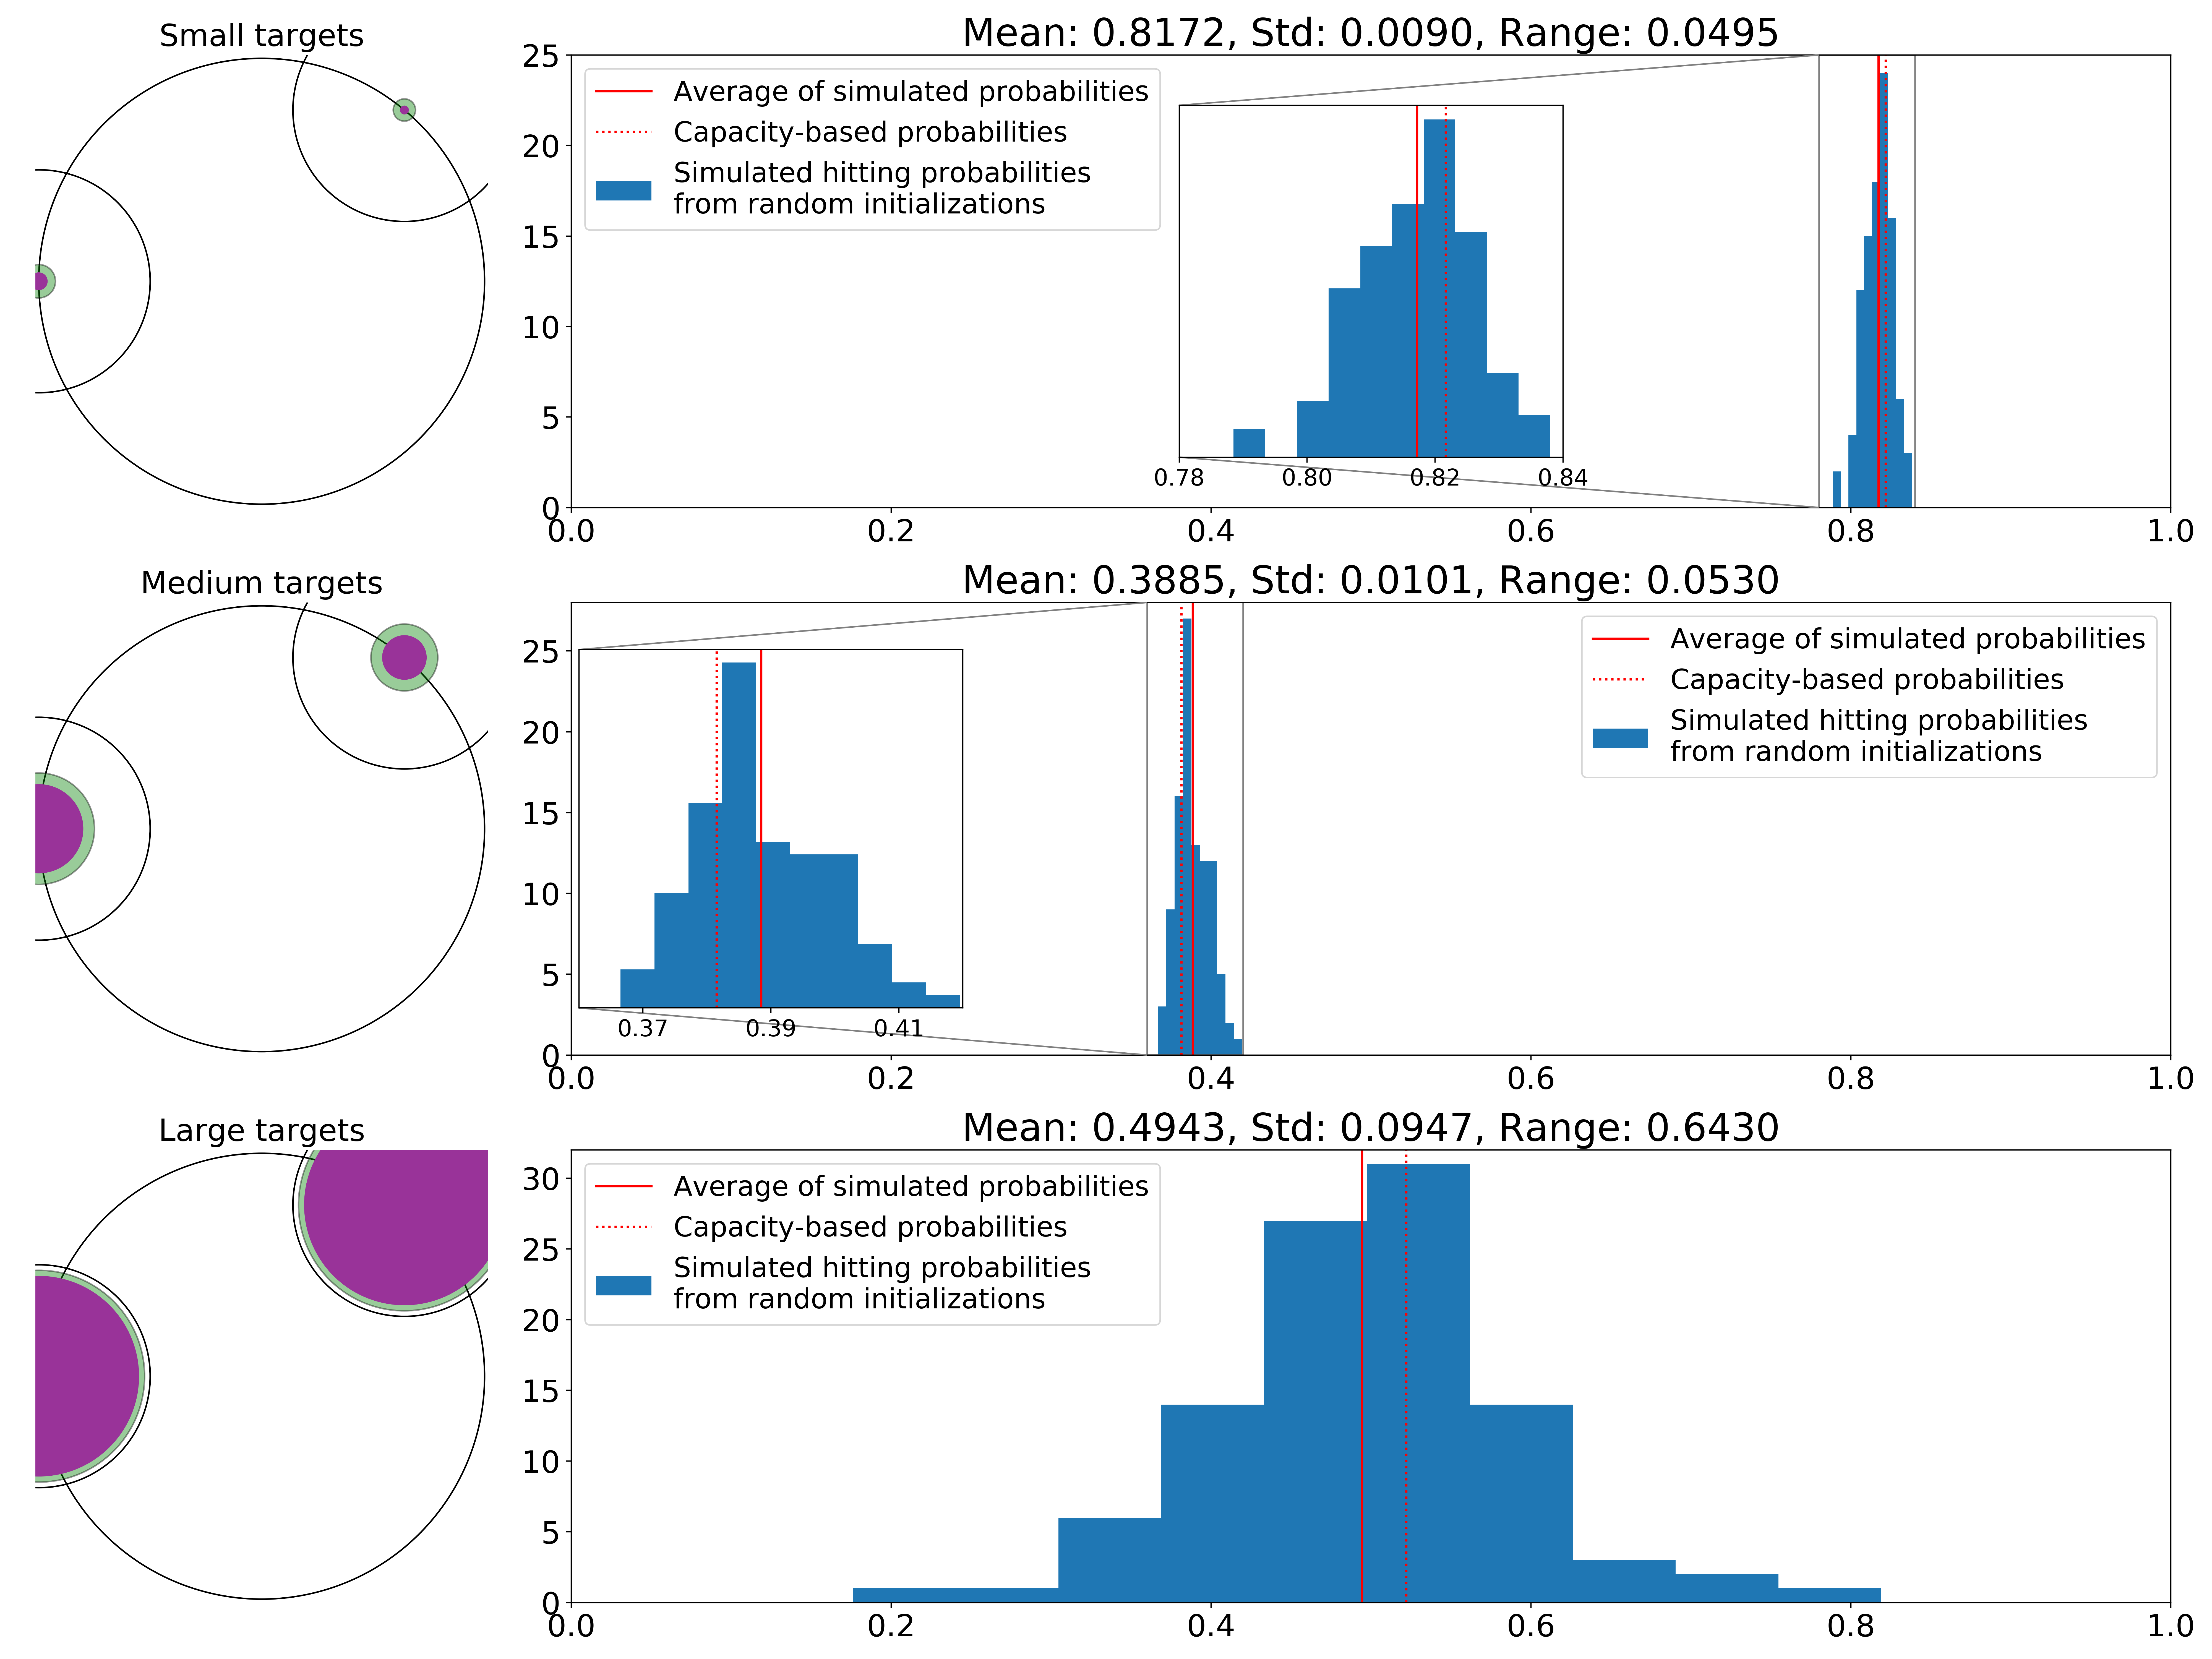
\includegraphics[width=\textwidth]{results_nontrivial.png}
    \caption{\label{fig:results_nontrivial} {\bf  Local capacities can accurately answer the question ``where will we go next?'' for nontrivial diffusions.}  The setup is similar to Figure \ref{fig:results_brownian_motion}, but now the targets $A$ and $B$ are only partially contained in $\Omega$ and the energy landscape becomes complicated near the targets. We again consider three different cases (small, medium and large targets), as illustrated in the left side of the figure. In each case, for each of 100 initial locations at modest distance from the targets, we estimate the probability of hitting target $A$ first.  In each case, we plot these 100 hitting probabilities with a histogram.  The histograms show that the first-passage probabilities vary significantly in the case of large targets, but they fall in a narrow range in the case of small and medium targets.  In all cases the capacity-based estimates, shown as dotted red lines, fall inside the span of the histograms.}
\end{minipage}}
\end{figure}

\subsection{Nontrivial Landscape}\label{sec:nontrivial_results}
The second set of experiments considers diffusions where the targets $A$ and $B$ are only partially contained in $\Omega$ and the energy landscape $U$ is nontrivial.  We fixed the target centers $x_A=(0.6402,0.7682,0.0,0,0,0.0), x_B=(-1.0,0.0,0.0,0,0,0.0)$ and the radii $r_\tA=r_\tB=0.5$.  We investigated three different cases with targets of different sizes: small (where $r_A=0.02, r_\dA=0.05, r_B=0.04, r_\dB=0.075$), medium (where $r_A=0.1, r_\dA=0.15, r_B=0.2, r_\dB=0.25$) and large (where $r_A=r_B=0.45, r_\dA=r_\dB=0.475$). More details of the specification can be found in Appendix \ref{sec:energy_function}. An illustration of the three different cases and the corresponding results are shown in Figure \ref{fig:results_nontrivial}.  We look at our three main questions in the context of these kinds of diffusions.

\subsubsection{Does the $\varepsilon$-flatness condition hold?}
Following the same procedure used in \S\ref{sec:toy_constant} we tested for the $\varepsilon$-flatness of $h_{A,B}$ on $M=\Omega\backslash(\tA\cup\tB)$. The histograms of the probabilities are illustrated in Figure \ref{fig:results_nontrivial}. We find that $h$ is $\varepsilon$-flat, with:
\begin{itemize}
    \item $\varepsilon\approx 0.0530$ when the targets are small
    \item $\varepsilon\approx 0.0495$ when the targets are medium
    \item $\varepsilon> 0.75$ when the targets are large
\end{itemize}
In the last case $h$ can hardly be called flat, varying by more than 75\% based depending upon the initial condition.  However, in the first two cases the constant $\varepsilon$ is sufficiently small that Theorem \ref{thm:main_thm} has relevant consequences.

\subsubsection{Are first-passage probabilities proportional to estimated capacities?}

Applying Theorem \ref{thm:main_thm} and using the shell method to estimate capacities, we can produce capacity-based estimates for the hitting probabilities.  These are shown as dotted red lines in Figure \ref{fig:results_nontrivial}.  Similar to the Brownian motion case, every hitting probability we looked at lay within $2\varepsilon/3$ of the capacity-based estimate.  This is better than the $\theepsrate$ promised by Theorem \ref{thm:main_thm} and closer to the minimum possible error of $\varepsilon/2$.   This again suggests that the bound of \ref{thm:main_thm} may be somewhat loose.

\subsubsection{Accuracy and speed of the shell method.}

How accurate is the shell method in this case?  In the previous section, we saw that we could use the shell-method to estimate capacities, use those capacities to get hitting-probability estimates, and that those estimates were fairly good.  This constitutes indirect evidence for the accuracy of the shell method.  However, this does not actually show that the shell-method accurately estimates the capacities (for example, if all estimated capacities were off by a multiplicative factor, this error would not show up in the estimates based on the shell method's capacity estimates).  Unfortunately, in this case it is not possible to obtain exact values for the capacity for this case, making it difficult to determine whether the shell algorithm is accurately estimating the capacity.   

Concerning computational efficiency: how fast is a capacity-estimation approach when compared against a simulation-based approach?  It is somewhat difficult to assess; there are many parameters and run times will depend on the dimension and details of the energies, possibly affecting the two approaches differently. In our experiments, for direct simulations we used the ``walk-on-spheres'' method to simulate trajectories in the flat region \cite{bingham1972random}, JIT compilation to remove loop overhead, multi-CPU parallelization, and the coarsest time step that yielded accurate results. As for capacity estimation, we made no effort to adjust the number of samples or the discretization parameters. 

Nonetheless, we can provide some facts which may give a sense for the computational efficiency gains.  Here are three different perspectives on the question:

\begin{description}
    \item[A single run of the direct simulation took about as long as estimating two capacities.]  Recall that estimating a hitting probability will require many runs of the direct simulation to see how often each target is hit.  

    \item[Getting a particular hitting probability with a 3\% error tolerance may be one-hundred times faster with capacities.]  In the small-targets Brownian motion case, the capacity-based estimate has a 3\% error.  That is, from any initial condition inside the set $M$, we found the true hitting probability to be within 3\% of the capacity-based estimate.  Now let us say we were interested in the hitting probability for a particular initial condition.  For some initial conditions the capacity-based estimator would actually be exactly correct.  However, for others it could be as much as 3\% off.  To achieve this 3\% error level using direct simulations we would need about 100 simulations (this follows from standard deviation of the binomial estimator for the hitting probability, together with the assumption that each individual simulation is exactly perfect).  As mentioned above, each simulation takes about as long as it does to compute both capacities.  Thus, if one wanted to compute the hitting probability up to within 3\% error, the capacity-based method would be one hundred times faster.

    \item[Estimating the mean hitting probability may be thousands of times faster with capacities.] Consider the problem of estimating the \emph{mean} hitting probability over the region $M$.  In other words, consider a diffusion initialized at a random location inside $M$: what is the probability it hits target $A$ first?  We measured these mean hitting probabilities for all of the examples above, using 200,000 different initial conditions; they are shown as solid red lines in Figures \ref{fig:results_brownian_motion} and \ref{fig:results_nontrivial}.   For example, in the medium-size target case, we find that the mean hitting probability was given by 38.93\%.  The capacity-based estimate was given by $38.15\%$.  This represents an error of $.8\%$.  To achieve a comparable error one would need to conduct about four thousand naive simulations.  
\end{description}


%  ____ ___ ____   ____ _   _ ____ ____ ___ ___  _   _
% |  _ \_ _/ ___| / ___| | | / ___/ ___|_ _/ _ \| \ | |
% | | | | |\___ \| |   | | | \___ \___ \| | | | |  \| |
% | |_| | | ___) | |___| |_| |___) |__) | | |_| | |\  |
% |____/___|____/ \____|\___/|____/____/___\___/|_| \_|



\section{Discussion}
\label{sec:Discussion}

If the hitting probability is nearly the same for every initial condition in a region $M$, then it can be well-approximated in terms of certain integrals.   We dub these integrals the ``first-passage capacities.''  These capacities can be approximately computed using a milestoning-like technique, as described in \S\ref{sec:Estimation}.  In Theorem \ref{thm:main_thm} we show that the error introduced by this approximation is small whenever hitting probabilities are fairly similar for different initial conditions inside a large region, $M$.  When this condition holds, we say the hitting probabilities are $\varepsilon$-flat; the coefficient $\varepsilon$ measures how much the hitting probabilities vary as one varies the initial condition.  Does this condition ever hold?  Can the hitting probabilities be similar for every initial condition in large region, $M$?  Theorem \ref{thm:epsilon_flat} shows several examples where the answer is yes.  Indeed, the answer is yes whenever the mixing rate of the diffusion is fast relative to the typical escape time from $M$.  In practice, this condition may not always be easy to check.

A major outstanding limitation of this work is that we provide no strategy for checking the $\varepsilon$-flatness condition.  In theory, bounds on the Lipschitz constant of the energy function and the Poincare constant for $M$ should be sufficient to ensure this condition, but we leave this for future work.  For now, we content ourselves that the condition certainly holds when the ambient dimension is at least three and the targets become small.  Moreover, when the dimension is very large then even targets with modestly large diameter can have very small overall volume, yielding a similar result.

The second major limitation of this work is that first-passage capacities do not directly inform us about the overall timescale on which the diffusion is operating.  The mean first-passage capacities are often inversely proportional to the first-passage times, but the overall proportionality constant is lost in this analysis.  In some limited cases, methods from the narrow escape literature may enable us to determine this overall constant.

In general, it may turn out that estimating first-passage times is profoundly more difficult than estimating first-passage hitting probabilities.  In this work we showed that the first-passage probabilities are sometimes invariant to the diffusion dynamics on the interior of a large set $M$, but the first-passing times will admit no such invariance.   If the dynamics inside of $M$ are genuinely intricate, it appears that estimating hitting times will always require a correspondingly intricate analysis.

We conclude by considering a possible future direction for this work.  Let us consider the case where we have many targets, $A_1,A_2\cdots A_n$, and the path between any two of the targets must pass through a set $M$.  In this case, assuming the $\varepsilon$-flatness condition holds on $M$, the order in which the process explores the targets could be accurately modeled using first-passage capacities alone.  In future we hope to explore this possibility.

\newpage
\appendix
\noindent {\bf APPENDIX}


%     _    ____  ____  _____ _   _ ____ _____  __     _
%    / \  |  _ \|  _ \| ____| \ | |  _ \_ _\ \/ /    / \
%   / _ \ | |_) | |_) |  _| |  \| | | | | | \  /    / _ \
%  / ___ \|  __/|  __/| |___| |\  | |_| | | /  \   / ___ \
% /_/   \_\_|   |_|   |_____|_| \_|____/___/_/\_\ /_/   \_\

\section{Three Perspectives on Hitting Probabilities}
\label{sec:three_perspectives}

Many of our results are based on the fact that hitting probabilities can actually be seen from three distinct perspectives.  To prepare for these results, we take a moment to review these three perspectives here.  Let $A,B\subset \Omega$, disjoint, open with smooth boundary.

\begin{enumerate}
\item Hitting probabilities.  Let $\tau_S \triangleq \inf\{t:\ X_t \in S\}$ for any set $S$ and $h_{A,B}(x) \triangleq \mathbb{P}(X_{\tau_{A\cup B}}\in \partial A|X_0=x)$.

\item Elliptic equation.  Let $h^\mathrm{dir}_{A,B}(x)$ denote the solution to the partial differential equation:
	    \begin{align}\label{eq:pde}
    0 &= \sum_{i = 1}^n b_i (x) \frac{\partial u
        (x)}{\partial x_i} + \frac{1}{2} \sum_{i = 1}^n \sum_{j = 1}^n a_{ij} (x)
        \frac{\partial^2 u (x)}{\partial x_i \partial x_j}\quad x\notin \bar A,\bar B\\
    1 &= u(x),x\in  A \nonumber \\
    0 &= u(x),x\in  B \nonumber \\
    0 &= \normal(x)^Ta(x)\nabla u(x), x \in \partial{\Omega}
    \nonumber
    \end{align}
This solution is unique and smooth.\cite{lieberman1986mixed}  What's more, it is equal to the hitting probability function: $h^\mathrm{dir}_{A,B}(x)=h_{A,B}(x)$ (cf.\ Section 6.7 of Chen\cite{chen2012symmetric}).
\item Variational form.  For any open set $S\subset \Omega$ let $\mathscr{E}_{S}(f,g)\triangleq \int_S \nabla f(x)^T a(x) \nabla g(x) \rho(dx)$ denote the ``Dirichlet Form'' of $f,g$ on the domain $S$.  Let $\mathscr L^2(S,\rho)$ denote the Hilbert space of functions on $S$ which are square-integrable with respect to $\rho$.  Let $\mathcal{H}^1(S,\rho)=W^{1,2}(S) \subset \mathscr{L}^2(S)$ denote the corresponding once-weakly-differentiable Hilbert Sobolev space.  We define $h^\mathrm{var}_{A,B}(x)$ as the solution to
    \begin{align*}
    \min_{u \in \mathcal H^1(S)} \quad & \mathscr{E}_S(u,u) \\
    \mbox{subject to} \quad & u(x)=1,x\in \partial A \\
     & u(x)=0,x\in \partial B
    \end{align*}
    where $S=\Omega \backslash (A\cup B)$.  This solution is unique and equal to $h^\mathrm{dir}_{A,B}$ on $S$ (cf.\ Section 4 of Dret\cite{dret2016partial}).
This variational perspective leads us to the notion of the ``condenser capacity'' associated with $h_{A,B}$.  It is defined as
    \[
    \capac{A}{\Omega \backslash B} \triangleq \mathscr{E}_S(h_{A,B},h_{A,B})
    \]
    where again $S=\Omega \backslash (A\cup B)=(\Omega \backslash B) \backslash A$.
\end{enumerate}
We will use all three of these perspectives to show our results.  For example, consider how the hitting probability perspective helps us show a result about capacities:
\begin{proposition}\label{prop:capacity}
Let $A\subset \tilde A,B\subset \tilde B$ with $\tilde A,\tilde B$ disjoint.  Then
\[
\capac{A\cup B}{\tilde A \cup \tilde B}=\capac{A}{\tilde A}+\capac{B}{\tilde B}
\]
\end{proposition}
\begin{proof}
This result is certainly known, but we include a proof here because we were unable to find a proof in the literature.  Since $\tilde A,\tilde B$ are disjoint and $X$ is continuous, the process cannot cross from one to the other without hitting the boundary.  Thus we have $\tau_{\partial \tilde A\cup \partial \tilde B \cup \partial A \cup \partial B}=\tau_{\partial \tilde A \cup \partial A}$ as long as $X_0\in\tilde A$.  We get a symmetric result if $X_0\in \tilde B$.  It follows that
\[
h_{A\cup B,(\tilde A\cup\tilde B)^c}(x) =
    \begin{cases}
    h_{A,\tilde A^c}(x) & \mbox{if }x\in \tilde A\\
    h_{B,\tilde B^c}(x) & \mbox{if }x\in \tilde B\\
    \end{cases}
\]
We can now use this probabilistic perspective to help us understand the capacity by articulating it as the Dirichlet form on the relevant hitting probability functions
\begin{align*}
\capac{A\cup B}{\tilde A \cup \tilde B}
        &= \int_{\tilde A\cup \tilde B \backslash (A\cup B)} \Vert \sigma \nabla h_{A\cup B,(\tilde A \cup \tilde B)^c}\Vert^2\rho(dx) \\
        &= \int_{\tilde A \backslash A} \Vert \sigma \nabla h_{A,\tilde A^c}\Vert^2\rho(dx)
            +\int_{\tilde B \backslash B} \Vert \sigma \nabla h_{B,\tilde B^c}\Vert^2 \rho(dx) \\
        &= \capac{A}{\tilde A}+\capac{B}{\tilde B}
\end{align*}
as desired.
\end{proof}

%     _    ____  ____  _____ _   _ ____ _____  __  ____
%    / \  |  _ \|  _ \| ____| \ | |  _ \_ _\ \/ / | __ )
%   / _ \ | |_) | |_) |  _| |  \| | | | | | \  /  |  _ \
%  / ___ \|  __/|  __/| |___| |\  | |_| | | /  \  | |_) |
% /_/   \_\_|   |_|   |_____|_| \_|____/___/_/\_\ |____/




\section{Proof of Theorem \ref{thm:epsilon_flat}}
\label{sec:proof_epsilon_flat}

\begingroup
\def\thetheorem{\ref{thm:epsilon_flat}}
\begin{theorem}
(Examples of $\varepsilon$-flatness).   Let $\bb{x,r} = \{y:\ \Vert x-y \Vert < r\}$ denote the ball of radius $r$ centered at $x$.  Recall that the process $X$ behaves according to the stochastic differential equation $dX_t = b(X_t)dt + \omega(X_t)dW_t$ contrained to lie inside a set $\Omega$ by normally reflecting boundaries.
\begin{enumerate}
    \item Let $\Omega \in \mathbb{R}^n, n\geq 3$ be convex and open with diameter less than or equal to 1.  Fix any points $x_A,x_B \in \mathbb{R}^n$.  For any $r,\varepsilon>0$ we can find $r'>0$ such that $h_{A,B}$ is $\varepsilon$-flat on $\Omega \backslash \bb{x_A,r}\cup \bb{x_B,r}$ for any $A\subset \bb{x_A,r'},B\subset \bb{x_A,r'}$ as long as $b(x)=0,\Omega(x)=I$ for $x \in \Omega \backslash \bb{x_A,r'}\cup\bb{x_B,r'}$.

    \item Fix $r,\varepsilon>0$ and also fix $r'<r$.  We can then find $n$ with the following property.  For any convex open set $\Omega \in \mathbb{R}^n$ with diameter less than or equal to 1, any $x_A,x_B$ such that $\bb{x_A, r},\bb{x_B, r} \subset \Omega$, and any $A\subset \bb{x_A, r'}, B \subset \bb{x_B, r'}$, we have that $h_{A,B}$ is $\varepsilon$-flat on $\Omega \backslash \bb{x_A, r} \cup \bb{x_B, r}$ as long as $b(x)=0,\Omega(x)=I$ for $x \in \Omega \backslash \bb{x_A,r'}\cup\bb{x_B,r'}$.
\end{enumerate}
\end{theorem}
\addtocounter{theorem}{-1}
\endgroup

\begin{proof}
Let $\dot A=\bb{x_A,r'},\dot B=\bb{x_B,r'}$.  Let $\{Z_t\}_t$ denote a Brownian motion trapped inside $\Omega$ and coupled to $X$ such that $X_{t}=Z_{t}$ for all $t\leq\tau=\left\{ \inf t:\ X_{t}\in\dot{A}\cup\dot{B}\right\} $ (we can do this because we assumed that $X$ behaves like Brownian motion outside of $\dot{A},\dot{B}$).  Let $Z_\infty$ denote the stationary distribution of $Z$, i.e. the uniform distribution on $\Omega$.
Using Lemma \ref{lem:uniform_ergodicity}, we have that
\[
\left|\mathbb{E}\left[h_{A,B}(Z_{t})-h_{A,B}(Z_{\infty}) | Z_0 =x \right]\right|\leq\frac{1}{t} \qquad \forall x
\]
On the other hand, Dynkin's formula gives that
\[
h_{A,B}(x)=\mathbb{E}\left[h_{A,B}(Z_{\tau\wedge t}) | Z_0=x\right]\qquad\forall t,x
\]
Putting those two facts together:
\begin{align*}
& \left|h_{A,B}(x)-\mathbb{E}\left[h_{A,B}(Z_{\infty})\right]\right| \\
=& \left|\mathbb{E}\left[h_{A,B}(Z_{\tau\wedge t})  - h_{A,B}(Z_{\infty}) | Z_0=x\right]\right|\\
 \leq & \left|\mathbb{E}\left[h_{A,B}(Z_{\tau\wedge t}) - h_{A,B}(Z_{t}) |Z_0=x\right]\right|+\left|\mathbb{E}\left[h_{A,B}(Z_{t}) -h_{A,B}(Z_{\infty}) | Z_0=x\right]\right|\\
 \leq& \mathbb{P}\left(\tau\leq t |Z_0 = x\right)+\frac{1}{t}
\end{align*}
To make this small, it thus suffices to get $t$ large but keep $\mathbb{P}\left(\tau\leq t\right)$ small.  In short, it suffices to show that $\tau$ is usually big.  We prove this differently in the two different cases:

\begin{enumerate}
    \item The first example follows because the targets are vanishing into nothing, so it is no surprise that the time to hit the targets will get longer and longer.  However, note that this intuition is valid only because  the ambient dimension $n$ is at least three (which we have assumed throughout).  A formal proof of this argument can be found in Lemma \ref{lem:longtime_diamater}.

    \item The second example is similar; even though the targets maintain the same diameter, their relative volume is vanishing because the ambient dimension $n$ is increasing.  Thus the targets are effectively becoming smaller, so the hitting time increases.  This matter is a bit trickier, and so for this second case note we have made additional requirements that $\bb{x_A,r},\bb{x_B,r} \subset \Omega$.  A formal proof of this argument can be found in Lemma \ref{lem:longtime}.
\end{enumerate}

\end{proof}

%%%%%%%%%%%%%%%%%%%%%%
%%%%%%%%%%%%%%%%%%%%%%

\begin{lemma}
\label{lem:uniform_ergodicity}(Uniform ergodicity) Let $\Omega\subset\mathbbm{R}^d$ be a convex set with diameter $\xi$ and let $M$ denote a Brownian motion trapped by reflecting boundaries inside $\Omega$.  The distribution of $M_t$ converges uniformly to the uniform distribution, in the sense that:
%
\[
\sup_{f:\ \Omega\rightarrow [0,1]} | \mathbb{E}[f(M_t) - f(Z)|M_0=x]| \leq \xi^2/4t \qquad \forall x\in \Omega, t>0
\]
%
where $Z$ is uniformly distributed on $\Omega$.
\end{lemma}
\begin{proof}
Per Loper \cite{Loper2018},
\[
\sup_{f:\ \Omega\rightarrow [0,1]} | \mathbb{E}[f(M_t) - f(Z)|M_0=x]| \leq \mathbbm{P}(\tau>4t)
\]
where $\tau$ is the first exit time of a one-dimensional Brownian motion from the interval $[-\xi,\xi]$ when initialized at the origin. Dynkin's formula gives that $\mathbb{E}[\tau]=\xi^2$. Hence, by the Markov inequality, $\mathbbm{P}(\tau>4t)\leq \xi^2/4t$.
\end{proof}

%%%%%%%%%%%%%%

\begin{lemma}
\label{lem:longtime_diamater}
Let Z denote a Brownian motion trapped inside a convex bounded open set $\Omega\subset\mathbb{R}^{n}$ with smooth boundary.  We further assume that $n\geq3$. Fix $x\in\mathbb{R}^{n}$ and $r,\epsilon>0$. Let $\tau_{A}$ denote $\inf\{t:\ Z_{t}\in A\}$ for any set A. We can always find $r_1>0$ such that $\mathbb{P}(\tau_{A}<1/\epsilon|Z_{0}=z)<\epsilon$ for all $z\notin\bb{x,r_3}$ and all $A\subset\bb{x,r_1}$.
\end{lemma}
\begin{proof}
First consider the case that $x \in \Omega$.  To measure the time it takes to hit $\bb{x,r_1}$, we will make use of two additional concentric spheres around $x$.  First, find $r_3$ such that $\bb{x,r_3} \subset \Omega$.  Second, let $r_2 =\sqrt{r_1 r_3}$, an intermediate radius.    We will use these spheres to break the trajectory of $Z$ into smaller manageable pieces. If $\left\Vert Z_{0}-x\right\Vert >r_3$,
the first part of the trajectory must carry it to a radius of $r_2$ before it reaches $r_1$.
The next part of the trajectory will then do one of two things: either
it will carry on to $r_1$ or it will first exit the ball of radius
$r_3$. Assuming it exits the ball of radius $r_3$, the strong Markov
property can be used to show that we are essentially in the same place
we started. Under this latter condition, the total time will be the
the time we've spent so far plus a new variable which has the same
properties as the original time. We can use this recursive relation to put a lower
bound on the overall time.

Let us make this rigorous. To measure the tails of $\tau$, we will
be interested in
\[
g(z)=\mathbb{E}\left[e^{-\frac{1}{2}\tau}|Z_{0}=z\right]
\]
To get a lower bound on the moments of $\tau$, we need to get an upper bound on this object.  To do so, we will use two objects of interest:
\begin{align*}
g_3 & =\sup_{z:\ \left\Vert z-x\right\Vert =r_3}g(z)\\
g_2 & =\sup_{z:\ \left\Vert z-x\right\Vert =r_2}g(z)
\end{align*}
using two stopping times of interest:
\begin{align*}
T_{2} & =\inf\{t:\ \Vert Z_{t}-x\Vert=r_2\}\\
T_{3} & =\inf\{t>T_{1}:\ \Vert Z_{t}-x\Vert=r_3\}
\end{align*}
Applying the strong Markov property, we observe that
\begin{align*}
g_{2} & =\sup_{z:\ \left\Vert z-x\right\Vert =r_2}\mathbb{E}\left[\mathbb{E}\left[e^{-\frac{1}{2}\tau}|Z_{T_{3}\wedge\tau}\right]|Z_{0}=z\right]\\
 & =\sup_{z:\ \left\Vert z-x\right\Vert =r_2}\mathbb{E}\left[e^{-\frac{1}{2}T_{3}\wedge\tau}g(Z_{T_{3}\wedge\tau})|Z_{0}=z\right]\\
 & \leq\sup_{z:\ \left\Vert z-x\right\Vert =r_2}\mathbb{E}\left[e^{-\frac{1}{2}T_{3}}g_{3}\mathbb{I}_{T_{3}<\tau}+e^{-\frac{1}{2}\tau}\mathbb{I}_{T_{3}>\tau}|Z_{0}=z\right]
\end{align*}
On the other hand, applying the continuity of Brownian motion we have
that $T_{2}<\tau$ whenever $Z_0$ lies outside the ball of radius $r_2$, so
\[
g_3=\sup_{z:\ \left\Vert z-x\right\Vert =r_3}\mathbb{E}\left[e^{-\frac{1}{2}T_{2}}g(T_{2})|Z_{0}=z\right]\leq g_2
\]
So in fact
\begin{align*}
g_3 & \leq\sup_{z:\ \left\Vert z-x\right\Vert =r_2}\mathbb{E}\left[e^{-\frac{1}{2}T_{3}}\mathbb{I}_{T_{3}<\tau}g_3+e^{-\frac{1}{2}\tau}\mathbb{I}_{T_{3}>\tau}|Z_{0}=z\right]\\
g_3 & \leq\frac{\sup_{z:\ \left\Vert z-x\right\Vert =r_2}\mathbb{E}\left[e^{-\frac{1}{2}\tau}\mathbb{I}_{T_{3}>\tau}|Z_{0}=z\right]}{1-\sup_{z:\ \left\Vert z-x\right\Vert =r_2}\mathbb{E}\left[e^{-\frac{1}{2}T_{3}}\mathbb{I}_{T_{3}<\tau}|Z_{0}=z\right]} = L
\end{align*}

To calculate this upper-bound $L$, defined above, Wendel gives explicit formulas (cf.\ \cite{Wendel1980-sj}).  We caution that in this document a somewhat nonstandard notation is used, namely Wendel uses $\mathbb{E}[A;B]$ to indicate $\mathbb{E}[A\times\mathbb{I}_B]$.  For any $z$ with $\Vert z-x\Vert=r_2$, Wendel uses the symmetry of the problem to show that
%
\begin{align*}
\mathbb{E}\left[e^{-\frac{1}{2}\tau}\mathbb{I}_{T_{3}>\tau}|Z_{0}=z\right]&=\left(\frac{r_{1}}{r_{2}}\right)^{h}\frac{I(r_{3})K(r_{2})-I(r_{2})K(r_{3})}{I(r_{3})K(r_{1})-I(r_{1})K(r_{3})}\\
\mathbb{E}\left[e^{-\frac{1}{2}\tau}\mathbb{I}_{T_{3}<\tau}|Z_{0}=z\right]&=\left(\frac{r_{3}}{r_{2}}\right)^{h}\frac{I(r_{1})K(r_{2})-I(r_{2})K(r_{1})}{I(r_{1})K(r_{3})-I(r_{3})K(r_{1})}
\end{align*}
%
where $h=(n-2)/2$ and $I,K$ denote the modified Bessel functions of order $h$.  This leads to the following explicit formula for $L$.
\begin{gather}
L=\frac{\left(\frac{r_{1}}{r_{2}}\right)^{h}\left(I_{3}K_{2}-I_{2}K_{3}\right)}{I_{2}K_{1}\left(\frac{I_{3}}{I_{2}}-\left(\frac{r_{3}}{r_{2}}\right)^{h}\right)+I_{1}K_{2}\left(\left(\frac{r_{3}}{r_{2}}\right)^{h}-\frac{K_{3}}{K_{2}}\right)}
\label{eq:Lforlongtime}
\end{gather}
where we denote $I_1=I(r_1),K_1=K(r_1),I_2=I(r_2)$, and so-on.  To prove our result, it thus suffices to show we can drive $L$ to zero by taking $n$ sufficiently large.

The numerator of $L$ in Equation (\ref{eq:Lforlongtime}) converges to zero as $r_1\rightarrow 0$, because $\frac{r_1}{r_2}\rightarrow 0,h>0$ and the other terms are constant.  On the other hand, the denominator explodes, because as $r_1\rightarrow0$ we have
\begin{align*}
\left(\frac{I_{3}}{I_{2}}-\left(\frac{r_{3}}{r_{2}}\right)^{h}\right)K_{1}I_{2}\rightarrow+\infty\\
\left(\left(\frac{r_{3}}{r_{1}}\right)^{h}-\frac{K_{3}}{K_{2}}\right)I_{1}K_{2}\rightarrow0
\end{align*}
These limits follow immediately from three properties of Bessel functions:
\begin{itemize}
    \item $K(x)\rightarrow \infty,I(x)\rightarrow 0$ as $x\rightarrow 0$ for $h>0$
    \item $K(x),I(x)>0$ for $x>0,h>0$
    \item $\frac{I(y)}{I(x)} > \left(\frac{y}{x}\right)^{h}$ for $y>x$ and $h>0$
\end{itemize}
The first two properties are well-known and can be found in DLMF (cf. \cite{noauthor_undated-ti}); the second can be found in Baricz (cf. \cite{noauthor_undated-ti,baricz2010bounds}). In conclusion, since the numerator vanishes and the denominator explodes, we have that overall $L$ vanishes.  Applying a Chernoff bound, we have our result for the case that $x \in \Omega$.

What happens if $x$ is not in the closure of $\Omega$?  Then by taking $r_1$ sufficiently small we can ensure that $A \cap \Omega = \emptyset$, so $\tau = \infty$.  Thus the result is proved automatically.

What if $x$ is precisely on the boundary of $\Omega$?  Here we must use the smoothness of the boundary of $\Omega$.  By picking $r_3$ sufficiently small, the smoothness guarantees that $\Omega$ is arbitrarily well-approximated by a half-plane when restricted to a ball $\bb{x,r_3}$.  In this half-plane case, identical arguments to the ones above can be used to argue that we can always take a $r_1$ that is yet smaller than $r_3$ and ensure that the hitting time is arbitrarily long.  Finally, to account for the slight discrepancy between the half-plane case and the actual case for some finite $r_3$, we appeal to the continuity of the Poisson equation which governs $g$ with respect to boundary condition (cf. \cite{strang1972approximation}).
\end{proof}


%%%%%%%%%%%%%%

\begin{lemma}
\label{lem:longtime} Fix $0<\epsilon$ and $0<r_1<r_3$.  Then we can always find an $n$ with the following property.  Pick any open set $\Omega \in \mathbb{R}^n$, any $x$ satisfying $\bb{x,r_3}\subset \Omega$, and any $x_0 \notin \bb{x,r_3}$.  Consider a Brownian motion $Z$ trapped inside $\Omega$ by reflecting boundaries and let $\tau$ denote the first hitting time of the process to $\bb{x,r_1}$.  Our choice of $n$ guarantees that
\[
\mathbb{P}(\tau < 1/\epsilon|Z_t=x_0) \leq \epsilon
\]
\end{lemma}
\begin{proof}
Following the same arguments found in Lemma \ref{lem:longtime_diamater}, we again obtain that $\mathbb{E}[e^{-\tau/2}|Z_0=x_0]$ is bounded by
\begin{gather}
L=\frac{\left(\frac{r_{1}}{r_{2}}\right)^{h}\left(I_{3}K_{2}-I_{2}K_{3}\right)}{I_{2}K_{1}\left(\frac{I_{3}}{I_{2}}-\left(\frac{r_{3}}{r_{2}}\right)^{h}\right)+I_{1}K_{2}\left(\left(\frac{r_{3}}{r_{2}}\right)^{h}-\frac{K_{3}}{K_{2}}\right)}
\end{gather}
To show our proof, it thus suffices to show we can drive this quantity to zero and then apply a Chernoff bound.

Let us first look at the numerator of $L$ in Equation \ref{eq:Lforlongtime}.  Asymptotics from the DLMF give that as $h \rightarrow \infty$ we have
\begin{align*}
I(x) \sim \frac{x^h}{2^h\Gamma(h+1)} & & K(x) \sim \frac{2^h\Gamma(h+1)}{(2h)x^h}
\end{align*}
Here by $f_1(h)\sim f_2(h)$ we mean ``asymptotic equivalence,'' i.e.\ $\lim_{h\rightarrow\infty}f_1(h)/f_2(h)=1$.  Plugging these in, we see that both terms in the numerator are asymptotically vanishing.

Now let us turn to the denominator.  Using the asymptotic formula above, we first note that
\begin{align*}
\left(\frac{r_{3}}{r_{2}}\right)^{h}I_{1}K_{2}&\sim\frac{1}{2h}\left(\frac{r_{3}r_{1}}{r_{2}^{2}}\right)^{h}=\frac{1}{2h}\rightarrow0\\
-\frac{K_3}{K_{2}}I_{1}K_{2}&\sim-\frac{1}{2h}\left(\frac{r_{1}}{r_{3}}\right)^{h}\rightarrow0
\end{align*}
So those terms are negligible.  However, the other two terms of the denominator are in fact exploding: one to positive infinity and one to negative infinity.  To understand this delicate balance, we these we turn to Lemma \ref{lem:bessel}.  Applying this Lemma and the asymptotics of the DLMF, we obtain that
\begin{align*}\left(\frac{I_{3}}{I_{2}}-\left(\frac{r_{3}}{r_{2}}\right)^{h}\right)K_{1}I_{2}&\geq\frac{r_{3}^{h}}{\cancel{I_{2}}}\times\frac{r_{3}^{2}-r_{2}^{2}}{2^{h+2}\Gamma(h+2)}K_{1}\cancel{I_{2}}\\
&\sim r_{3}^{h}\times\frac{r_{3}^{2}-r_{2}^{2}}{2^{h+2}\Gamma(h+2)}\frac{2^{h}\Gamma(h+1)}{2hr_{1}^{h}}\\&=\left(\frac{r_{3}}{r_{1}}\right)^{h}\left(\frac{r_{3}^{2}-r_{2}^{2}}{8h(h+1)}\right)
\end{align*}
which is indeed exploding to positive infinity as $h=(n-2)/2 \rightarrow \infty$.

Thus, since the numerator vanishes and the denominator explodes to positive infinity, we have that $L$ vanishes as $n\rightarrow \infty$.
\end{proof}

\begin{lemma}\label{lem:bessel}
Let $I$ denote the modified bessel function of the first kind of order $h$.  If $a>b$ then
    \[
    \frac{I ( a)}{I (b)} - \left(\frac{a}{b} \right)^h
    \geq
    \frac{a^h}{I(b)}\times\frac{a^{2} -b^{2}}{2^{h+2}\Gamma(h+2)}
    \]
\end{lemma}
\begin{proof}
Recall that $I$ may be defined as
\[
I(x) = \sum_{m=0}^\infty \frac{x^{h+2m}}{2^{h+2m}\Gamma(m+h+1)\Gamma(m+1)}
\]
Thus
\begin{align*}
\frac{I ( a)}{I (b)} - \left(\frac{a}{b} \right)^h
    &= \frac{I(a)b^h-a^hI(b)}{b^hI(b)}  \\
    &= \frac{a^hb^h\sum_{m=0}^\infty \frac{a^{2m} -b^{2m}}{2^{h+2m}\Gamma(m+h+1)\Gamma(m+1)}}{b^{h}I(b)}
\end{align*}
Since $a>b$, we have that $a^{2m} -b^{2m}$ is always positive.  Thus we can get a lower bound by simply taking one of the terms.  Choosing $m=1$, we get our final result.
\end{proof}

%  ____ _____     _______ ____   ____ _____ _   _  ____ _____
% |  _ \_ _\ \   / / ____|  _ \ / ___| ____| \ | |/ ___| ____|
% | | | | | \ \ / /|  _| | |_) | |  _|  _| |  \| | |   |  _|
% | |_| | |  \ V / | |___|  _ <| |_| | |___| |\  | |___| |___
% |____/___|  \_/  |_____|_| \_\\____|_____|_| \_|\____|_____|



\section{Proof of Theorem \ref{thm:main_thm}}
\label{sec:proof_thm}

Let $A\subset\tilde A\subset\Omega,B\subset\tilde B\subset\Omega$.  Let $\tilde A,\tilde B$ be disjoint and
$h_{A,B}(x)$  $\varepsilon$-flat with respect to $\Omega \backslash (\tilde A \cup \tilde B)$. We assume the set boundaries are all smooth.

Under these conditions, we will show we can use local capacities to get good approximations for $h_{A,B}(x)$ when $x\notin \tilde A,\tilde B$.  To do so, our key idea is to uncover upper and lower bounds on the value of the Dirichlet form applied to this function, $\mathscr{E}(h_{A,B},h_{A,B})$.  We will see that these bounds can be understood in terms of local capacities, and the resulting inequalities will then yield our main result in the form of Theorem \ref{thm:main_thm}.

\begin{lemma}  Let $S=\Omega \backslash (A\cup B)$.  The Dirichlet form of $h_{A,B}$ on $S$ can be upper-bounded in terms of the capacities:
\[ \mathscr{E}_S(h_{A,B}, h_{A,B}) \leqslant \frac{\tmop{cap} (A, \tilde{A}) \tmop{cap} (B,
\tilde{B})}{\tmop{cap} (A, \tilde{A}) + \tmop{cap} (B, \tilde{B})} \]
\end{lemma}
\begin{proof}
We recall from Appendix \ref{sec:three_perspectives} that
%
\[
\mathscr{E}_S(h_{A,B}, h_{A,B}) = \capac{A}{\Omega \backslash B} \leq \mathscr{E}_S (u,u)
\]
%
for any $u$ with $u(\partial A) = 1,u(\partial B) = 0$.  Thus, to prove an upper bound it suffices to find any such function for which we can calculate $\mathscr{E}(u,u)$.  To this end, consider
%
\[
u_c (x) \triangleq \left\{ \begin{array}{ll}
(1 - c) h_{A, \widetilde{A}^c} (x) + c & \tmop{if} x \in \tilde{A} \\
c (1 - h_{B, \widetilde{B}^c} (x)) & \tmop{if} x \in \tilde{B} \\
c & \mbox{otherwise}
\end{array} \right.
\]
%
These functions are well-suited to giving us upper bounds on $\mathscr{E}_S (h_{A,B}, h_{A,B})$.  Indeed:
\begin{itemize}
\item $u_c(\partial A)=1,u_c(\partial B)=0$.  In fact, $u_c$ takes a constant value $c$ outside of $\tilde A,\tilde B$, drops smoothly in $\tilde B$ to achieve 0 on $\partial B$, and rises smoothly in $\tilde A$ to achieve 1 on $\partial \tilde A$.
\item Noting that $u_c$ is written as a piecewise combination of hitting probability functions, we see that its Dirichlet form can be calculated in terms of capacities on local regions: $\mathscr{E}_S(u_c,u_c) = (1 - c)^2 \tmop{cap} (A, \tilde{A}) + c^2 \tmop{cap} (B, \tilde{B})$.
\end{itemize}
Thus the $u_c$ functions give us a practical way to calculate upper bounds:
\[
\mathscr{E}_S(h_{A,B}, h_{A,B})\leq (1 - c)^2 \tmop{cap} (A, \tilde{A}) + c^2 \tmop{cap} (B, \tilde{B})
\]
This inequality holds for any value of $c$.  To get the best bound, we can take derivatives to minimize the right hand side with respect to $c$.  The result is
\[
c^* = \frac{\capac{A}{\tilde A}}{\capac{A}{\tilde A}+\capac{B}{\tilde B}}
\]
Plugging this into the previous equation, we obtain our final result.
\end{proof}

%%%%%%%%%%%
%%%%%%%%%%%

\begin{lemma}  Let $S=\Omega \backslash (A\cup B)$.  Let $m = \frac{1}{2} (\sup_{x \notin \tilde A,\tilde B} h_{A,B} (x) + \inf_{x \notin \tilde A,\tilde B} (h_{A,B} (x)))$.  The Dirichlet form of $h_{A,B}$ can be lower-bounded in terms of $m$ and the capacities:
\[\mathscr{E}_S (h_{A,B}, h_{A,B}) \geq
   \left( 1 - m - \frac{\varepsilon}{2} \right)^2 \tmop{cap} (A,\tilde{A}) \indicatorf{m\leq 1-\frac{\varepsilon}{2}} +
   \left( m- \frac{\varepsilon}{2} \right)^2 \tmop{cap} (B, \tilde{B})\indicatorf{m\geq \frac{\varepsilon}{2}}
\]
\end{lemma}
\begin{proof}
Recall that $\mathscr{E}_S(h_{A,B}, h_{A,B})$ can be expressed as an integral over $S$.  We decompose this into three integrals: one over $\tilde A$, one over $\Omega \backslash \tilde A,\tilde B$, and one over $\tilde B$.
\[
\mathscr{E}_S (h_{A,B}, h_{A,B}) = \int_{\tilde A \backslash A} \Vert \sigma \nabla h_{A,B}\Vert^2 \rho(dx)
                                 + \int_{\tilde B \backslash B} \Vert \sigma \nabla h_{A,B}\Vert^2 \rho(dx)
                                 + \int_{\Omega \backslash \tilde A,\tilde B} \Vert \sigma \nabla h_{A,B}\Vert^2 \rho(dx)
\]
Since the integrand is always positive, we can get a lower bound by simply ignoring the integral over $\Omega \backslash \tilde A,\tilde B$ and focusing on the integrals over $\tilde A,\tilde B$.  The $\tilde A,\tilde B$ integrals can be lower-bounded using capacities.

For example, let us focus on the $A$ integral.  There are two different possibilities we must consider:
\begin{itemize}
\item If $m>1-\varepsilon/2$ we will simply note that the integral over the $\tilde A$ region is non-negative.
\item If $m\leq 1-\varepsilon/2$, then we define
    \[
    u_A (x) \triangleq \frac{h_{A,B} (x) - m - \frac{\varepsilon}{2}}{1 - m - \frac{\varepsilon}{2}}
    \]
    Note that  $h_{A,B}(x)=1$ for $x \in \partial A$ and the $\varepsilon$-flatness condition shows that $h_{A,B}(x) \leq m + \frac {\varepsilon}{2}$ for $x \in \partial \tilde A$.  Thus $u_A(\partial A)\geq1,u_A(\partial \tilde A)\leq 0$.  Lemma \ref{lem:inequalityboundaryvar} from Appendix \ref{sec:inequalityboundaryvar} may then be applied to yield that $\mathscr{E}_{\tilde A \backslash A}(u_A,u_A) \geq \capac{A}{\tilde A}$.  We can thus obtain the bound
    \begin{align*}
    \int_{\tilde A \backslash A} \Vert \sigma \nabla h_{A,B}\Vert^2 \rho(dx)
	 &= \left(1 - m - \frac{\varepsilon}{2}\right)^2 \mathscr{E}_{\tilde{A} \backslash A}(u_A,u_A)\\
         &\geq \left(1 - m - \frac{\varepsilon}{2}\right)^2 \capac{A}{\tilde A}
    \end{align*}
\end{itemize}
Putting these two possibilities together, we obtain
\[
\int_{\tilde A \backslash A} \Vert \sigma \nabla h_{A,B}\Vert^2 \rho(dx) \geq \left(1 - m - \frac{\varepsilon}{2}\right)^2 \capac{A}{\tilde A}\indicatorf{m\leq 1-\frac{\varepsilon}{2}}
\]
Applying the same ideas to the integral over $\tilde B$, we obtain our result.
\end{proof}

%%%%%%%%%%%
%%%%%%%%%%%

We are now in a position to prove Theorem \ref{thm:main_thm} from the main text:

\begingroup
\def\thetheorem{\ref{thm:main_thm}}
\begin{theorem}
Assume that  $h_{A,B}(x)$ is $\varepsilon$-flat relative to
$\Omega \backslash (\tilde A \cup \tilde B)$.
Then the first-passage probabilities can be well-approximated in terms of the target capacities:
\[ \sup_{x \notin \tilde A,\tilde B} \left| h_{A,B} (x) - \frac{\capac{A}{\tilde A}}{\capac{A}{\tilde A}+\capac{B}{\tilde B}} \right| \leqslant \varepsilon + \sqrt{\varepsilon/2} \]
\end{theorem}
\addtocounter{theorem}{-1}
\endgroup


\begin{proof}

To simplify notation, let $\capA=\capac{A}{\tilde A}$ and $\capB=\capac{B}{\tilde B}$.  Applying the previous two lemmas together, we obtain the inequality
\[
\frac{\capA \capB}{\capA +\capB}
\geq \mathscr{E}(h_{A,B},h_{A,B}) \geq
\left( 1 - m - \frac{\varepsilon}{2} \right)^2 \capA \indicatorf{m\leq 1-\frac{\varepsilon}{2}} +
   \left( m- \frac{\varepsilon}{2} \right)^2 \capB \indicatorf{m\geq \frac{\varepsilon}{2}}
\]
where $m = \frac{1}{2} (\sup_{x \notin \tilde A,\tilde B} h_{A,B} (x) + \inf_{x \notin \tilde A,\tilde B} (h_{A,B} (x)))$.  In analyzing this inequality, there are three possibilities to consider.
\begin{itemize}
    \item If $m \in (\varepsilon/2,1-\varepsilon/2)$, the quadratic formula yields
    \begin{eqnarray*}
    m & \geqslant & \frac{\capA}{\capA + \capB} + \frac{
    \frac{\varepsilon}{2}(\capB - \capA) -
    \sqrt{\capA \capB \varepsilon( 2 - \varepsilon)}}{\capA+\capB}\\
    m & \leqslant & \frac{\capA}{\capA + \capB} + \frac{
    \frac{\varepsilon}{2}(\capB - \capA) +
    \sqrt{\capA \capB \varepsilon( 2 - \varepsilon)}}{\capA+\capB}
    \end{eqnarray*}
    Applying $\left|\frac{\capB - \capA}{\capA + \capB}\right| \leq 1$ and the fact that the geometric mean $\sqrt{\capA \capB}$ never exceeds the arithmetic mean $(\capA+\capB) / 2$, it follows that
    \[
    \left|m -  \frac{\capA}{\capA + \capB}\right| \leq \frac{\varepsilon +\sqrt{\varepsilon (2-\varepsilon)}}{2}
    \]
    Applying the fact that $m$ was designed so that $|h_{A,B}(x) - m| <\varepsilon/2$ for all $x \notin \tilde A,\tilde B$, we obtain
    \[
    \left|h_{A,B}(x) -  \frac{\capA}{\capA + \capB}\right| \leq \frac{2\varepsilon +\sqrt{\varepsilon (2-\varepsilon)}}{2}
    \]

    \item If $m<\varepsilon/2$, our equations become
    \[
    \frac{\cancel{\capA} \capB}{\capA +\capB}
    \geq
    \left( 1-m- \frac{\varepsilon}{2} \right)^2 \cancel{\capA}
    \]
    Our assumption that $m \leq \varepsilon/2$ indicates that $(1- m- \varepsilon/2)^2 \geq (1-\varepsilon)^2$, thus in fact we have
    \[
    \frac{\capB}{\capA +\capB}
    \geq
    \left( 1- \varepsilon \right)^2  = 1 + \varepsilon^2 - 2\varepsilon
    \]
    which means that $\capA/(\capA +\capB)
    \leq
    2\varepsilon - \varepsilon^2 \leq 2\varepsilon$.
    Thus we assumed $m\in[0,\varepsilon/2]$ and showed that $\capA/(\capA+\capB)\in[0,2\varepsilon-\varepsilon^2]$, so it follows that
    \[
    \left|m -  \frac{\capA}{\capA + \capB}\right| \leq 2\varepsilon -\varepsilon^2
    \]
    and so for any $x\notin \tilde A,\tilde B$, we have
    \[
    \left|h_{A,B}(x) -  \frac{\capA}{\capA + \capB}\right| \leq 2.5\varepsilon -\varepsilon^2
    \]

    \item If $m>1-\varepsilon/2$, the same bound can be achieved by arguments which are symmetric to those employed in $m<\varepsilon/2$:
    \[
    \left|h_{A,B}(x) -  \frac{\capA}{\capA + \capB}\right| \leq 2.5\varepsilon -\varepsilon^2
    \]
\end{itemize}
Our final result is found by noting that all these bounds are upper-bounded by $\varepsilon + \sqrt{\varepsilon/2}$.
\end{proof}

%     _    ____  ____  _____ _   _ ____ _____  __   ____
%    / \  |  _ \|  _ \| ____| \ | |  _ \_ _\ \/ /  / ___|
%   / _ \ | |_) | |_) |  _| |  \| | | | | | \  /  | |
%  / ___ \|  __/|  __/| |___| |\  | |_| | | /  \  | |___
% /_/   \_\_|   |_|   |_____|_| \_|____/___/_/\_\  \____|





\section{Proof of Proposition \ref{prop:flux}}
\label{sec:proof_proposition}

We first establish a lemma, using Green's first identity and some properties of the stationary SDE (\ref{equ:general_sde}), under the reversibility conditions (\ref{eqn:reversibility}), relative to $U$:

\begin{lemma}  \label{lem:greenident}Fix some $S \subset \Omega$ with smooth boundary.  Then for any smooth function $g$ that satisfies $\mathcal{L}g = 0$ and smooth function $f$,
\begin{equation*}
\int_{S} \nabla f(x)^T a(x) \nabla g(x) e^{-U(x)}dx = \int_{\partial S} f(x) \normal(x)^T a(x) \nabla g(x) e^{-U(x)}\hausdorffmeasure
\end{equation*}
where $\normal$ are the normal vectors facing out of the set $S$ and $\hausdorffmeasure$ is the integral with respect to the $(n-1)$-dimensional Hausdorff measure and
\[
(\mathcal{L}f)(x) \triangleq \sum_i b_i(x) \frac{\partial f (x)}{\partial x_i} +
    \frac{1}{2} \sum_{ij}a_{ij}(x)\frac{\partial^2 f(x)}{\partial x_i \partial x_j}
\]
\end{lemma}
\begin{proof}
This result is essentially a direct corollary of Green's identities.  Apply Green's first identity to get
\begin{align*}
	 &\int_{S} \nabla f^T a \nabla g e^{-U} dx\\
	=&\int_{\partial S}f \normal^T a \nabla g e^{-U} \hausdorffmeasure - \int_{S} f \nabla \cdot (a \nabla g e^{-U}) dx
\end{align*}
where
\begin{equation*}
	\nabla \cdot (a \nabla g e^{-U}) = \sum_{i}\frac{\partial}{\partial x_i}\left[\sum_{j}e^{-U}a_{i j}\frac{\partial g}{\partial x_j}\right]
\end{equation*}
Next, using the reversibility constraint on $b$ from Equation (\ref{eqn:reversibility}), it's not hard to verify that
\begin{equation*}
	\nabla \cdot (a \nabla g e^{-U}) = 2e^{-U}\mathcal{L} g = 0
\end{equation*}
This gives us the desired result.
\end{proof}

\def\theproposition{\ref{prop:flux}}
\begin{proposition}
For any regions $G$ and $\tilde{G}$ having smooth boundaries and such that $A\subset G \subset \tilde G \subset \tilde A$, $\capac{A,\tA}$ can be expressed as a flux leaving $\tilde G \backslash G$:
\[
\ensuremath{\operatorname{cap}} (A, \tilde{A}) = \int_{\partial (\tilde G \backslash G)}  h_{A, \tilde{A}^c} (x)   \normal(x)^T a (x) \nabla h_{G, \tilde{G}^c} (x)e^{- U (x)} \hausdorffmeasure
\]
where $a(x)=\sigma(x)\sigma(x)^T$ is the diffusion matrix, $\hausdorffmeasure$ is the $(n-1)$-dimensional Hausdorff measure, and $\normal$ represents the outward-facing (relative to $\tilde G \backslash G$) normal vector on $\partial (\tilde G \backslash G)$.
\end{proposition}
\addtocounter{proposition}{-1}
\begin{proof}
This result is certainly known, but we include a proof here because we were unable to find a proof in the literature.  First recall that $\mathcal{L} h_{A, \tilde{A}^c} = 0$ and
\begin{equation*}
	\tmop{cap}(A,\tilde A) = \int_{\tilde A \backslash A} \nabla h_{A, \tilde{A}^c} (x)^T a(x) \nabla h_{A, \tilde{A}^c} (x) e^{-U(x)} dx
\end{equation*}
Together with Lemma \ref{lem:greenident}, this yields that
\begin{equation}\label{eq:lemmaproof}
\tmop{cap}(A,\tilde A)  = \int_{\partial (\tilde A \backslash A)}  h_{A, \tilde{A}^c} \normal^T a  \nabla h_{A, \tilde{A}^c} e^{- U } \hausdorffmeasure = -\int_{\partial A}  \normal^T a  \nabla h_{A, \tilde{A}^c} e^{- U } \hausdorffmeasure
\end{equation}
where in the last step we used $h_{A,\tilde A^c}(x)=1,x\in \partial A,h_{A,\tilde A^c}(x)=0,x\in \partial \tilde A$.  Also, note that the normal vector on the right hand side is pointing {\em out of} the set $A$, as is our convention. Hence then negative sign.

Next we apply Lemma \ref{lem:greenident} again to get
\begin{align*}
	0 = \int_{G \backslash A} \cancel{\nabla (1)} a \nabla h_{A,\tilde A^c}^T e^{- U } dx = \int_{\partial (G\backslash A)} \normal^T a  \nabla h_{A,\tilde A^c} e^{- U } \hausdorffmeasure
\end{align*}
Combining this with Equation \ref{eq:lemmaproof} gives us
\begin{equation}
\label{eqn:cor}
\tmop{cap}(A,\tilde A)  = -\int_{\partial A}  \normal^T a  \nabla h_{A, \tilde{A}^c} e^{- U } \hausdorffmeasure = \int_{\partial G}  \normal^T a  \nabla h_{A, \tilde{A}^c} e^{- U } \hausdorffmeasure
\end{equation}
Using the facts that $h_{G,\tilde G^c}(x)=1,x\in \partial G,h_{G,\tilde G^c}(x)=0,x\in \partial \tilde G$, and $\mathcal{L} h_{G, \tilde G^c} = 0$, we apply Lemma \ref{lem:greenident} two more times to obtain
\begin{align*}
	\tmop{cap}(A,\tilde A)  &= \int_{\partial G}  \normal^T a  \nabla h_{A, \tilde{A}^c} e^{- U } \hausdorffmeasure = \int_{\partial G}  h_{G, \tilde{G}^c} \normal^T a   \nabla h_{A, \tilde{A}^c} e^{- U } \hausdorffmeasure\\
				&= \int_{\partial (\tilde G \backslash G)}  h_{G, \tilde{G}^c} \normal^T a   \nabla h_{A, \tilde{A}^c} e^{- U } \hausdorffmeasure
				= \int_{\tilde G \backslash G}  \nabla h_{G, \tilde{G}^c} a \nabla h_{A, \tilde{A}^c} e^{- U } dx\\
				&= \int_{\partial (\tilde G \backslash G)}  h_{A, \tilde{A}^c}    \normal^T a  \nabla h_{G, \tilde{G}^c} e^{- U } \hausdorffmeasure
\end{align*}
\end{proof}

\begin{corollary*}
%\label{cor:flux}
For any region $S$ having smooth boundary $\partial S$, and such that $A\subset S \subset \tilde A$, $\capac{A,\tA}$ can be expressed as a flux leaving $S$:
\begin{equation*}
\ensuremath{\operatorname{cap}} (A, \tilde{A}) = \int_{\partial S}   \normal(x)^T a (x) \nabla h_{A, \tilde{A}^c} (x)e^{- U (x)} \hausdorffmeasure
\end{equation*}
where $a$ and $\hausdorffmeasure$ are as defined in the Proposition, and  $\normal$ is the outward-facing normal on $\partial S$.
\end{corollary*}
\begin{proof}
Put $G=S$ in Equation (\ref{eqn:cor}).
\end{proof}

%
%
%
%
%
%
%
%
%
%
\section{Inequality Boundary Conditions for the Variational Form}
\label{sec:inequalityboundaryvar}

Recall that $h_{A,B}(x)$ may be defined variationally.  We have let
%
\[
\mathscr{E}(f,g)\triangleq \int_\Omega \nabla f(x)^T a(x) \nabla g(x) \rho(dx)
\]
%
denote the ``Dirichlet Form.''  Let $\Omega \subset \mathbb{R}^n$ compact and open with smooth boundary.  Let $\mathscr L^2(\bar \Omega,\rho)$ denote the Hilbert space of functions on $\bar \Omega$ which are square-integrable with respect to a continuous positive measure $\rho(dx)=e^{-U}dx$.  Let $\mathcal{H}^1(\bar \Omega,\rho)=W^{1,2}(\bar \Omega,\rho) \subset \mathscr{L}^2(\bar \Omega,\rho)$ denote the corresponding once-weakly-differentiable Hilbert Sobolev space.  Let $A,B\subset \Omega$, open, disjoint, with smooth boundary, and define $\capac{A}{\Omega \backslash B} \in \mathbb{R}$ as the minimizing value of the problem
    \begin{align*}
    \min_{u \in \mathcal H^1} \quad & \mathscr{E}(u,u) \\
    \mbox{subject to} \quad & u(x)=1,x\in A \\
     & u(x)=0,x\in B
    \end{align*}

It is natural to consider an apparently different problem, where the equality boundary conditions are replaced with inequalities.  Here we show that it is not possible to get lower than $\capac{A}{\Omega \backslash B}$ by such a relaxation.

\begin{lemma} \label{lem:inequalityboundaryvar} Let $\tilde h$ satisfy $\tilde h(x)\geq 1$ on $A$ and $\tilde h(x)\leq 0$ on $B$.  Then $\mathscr{E}(\tilde h,\tilde h) \geq \capac{A}{\Omega \backslash B}$.
\end{lemma}
\begin{proof}
This result is certainly known, but we include a proof here because we were unable to find a proof in the literature.  Let $k=\mathtt{clamp}(\tilde h,0,1)$, i.e.
\[
k(x)=
\begin{cases}
\tilde h(x) & \tilde h(x)\in[0,1] \\
0 & \tilde h(x)\leq 0 \\
1 & \tilde h(x)\geq 1 \\
\end{cases}
\]
Note that $k\in \mathcal{H}^1$ and satisfies the equality boundary conditions.  Thus, by definition, $\capac{A}{\Omega \backslash B} \leq \mathscr{E}(k,k)$.  This immediately yields our result:
\begin{align*}
\capac{A}{\Omega \backslash B} \leq \mathscr{E}(k,k) &= \int \Vert \sigma \nabla k \Vert^2 \rho(dx) \\
    &=\int_{x:\ \tilde h(x)\in[0,1]} \Vert \sigma \nabla \tilde h \Vert^2 \rho(dx) \\
    &\leq \int \Vert \sigma \nabla \tilde h \Vert^2 \rho(dx) = \mathscr{E}(\tilde h,\tilde h)
\end{align*}


% Let us look at the properties of their difference, $k=\tilde h- h$.
% \begin{itemize}
%     \item $\mathscr{E}(k,k)=\mathscr{E}(h,h)+\mathscr{E}(\tilde h,\tilde h)+2\mathscr{E}(h,\tilde h)$
%     \item $k(A)\geq 0$
%     \item $k(B)\leq 0$
% \end{itemize}
\end{proof}

%
%
%
%
%
%
%
%
%






\section{Shell Method}
\label{sec:shell_method}

The algorithm for estimating local hitting probabilities is outlined as follows:

{\algorithm{\label{alg:hitting_prob_estimation}Estimating $h_{R,\tilde R^c}(x)$ for many values of $x$ on a shell $\partial S$

\begin{description}
    \item[Input] $R \subset S \subset \tilde{R} \subset \Omega$ and a stationary reversible  diffusion process $\{X_t\}_{t \geq 0}$ in $\Omega$ with invariant measure ${\mu}= e^{- U (x)} \mathrm{d} x$. We also require a series of subsets
  \[ R = S_0 \subset S_1 \subset \cdots \subset S_{m - 1}
     \subset S_m = S \subset S_{m + 1} \subset \cdots \subset S_n = \tilde{R} \]
     which indicate a kind of reaction coordinate.

    \item[Output] A collection of points $z_1,\cdots z_{N_p}$ on $\partial S$ sampled from the invariant measure ${\mu}= e^{- U (x)} \mathrm{d} x$ restricted on $\partial S$, along with estimates of $h_{R,\tilde R^c}(z_i)$ for each point.

\end{description}

\begin{enumerate}
\item Discretize the space.
\begin{enumerate}
  \item Generate an ensemble of samples $z_1, \ldots, z_{N_p}$ on $\partial S$
  according to the invariant measure ${\mu}= e^{- U (x)} \mathrm{d} x$ restricted to $\partial S$.

  \item Evolve the ensemble on $\partial S$, by repeatedly sampling an initial location from the uniform distribution on $\{ z_1, \ldots, z_{N_p} \}$ and carry out a local simulation following the dynamics of $\{X_t\}_{t \geq 0}$
  until the trajectory hits either $\partial S_{m - 1}$ or $\partial S_{m +
  1}$. Record the hitting locations on $\partial S_{m - 1}$ and $\partial S_{m + 1}$ until we have $N_p$ points on both $\partial S_{m - 1}$ and $\partial
  S_{m + 1}$. In most cases, the process is more likely to hit one of $S_{m - 1}, S_{m + 1}$ than the other, and we need to run more than $2N_p$ local simulations to get at least $N_p$ samples on both shells. We store the results of the redundant local simulations for future estimation of transition probabilities.

  \item Repeat the above process to sequentially evolve the ensembles on $\partial S_{m - 1}, \ldots,
  \partial S_2$ and on $\partial S_{m + 1}, \ldots, \partial S_{n - 2}$, to get $N_p$ samples on all of the intermediate shells $\partial S_1,
  \ldots, \partial S_{n - 1}$. Store the results of the redundant local simulations for future
  estimation of transition probabilities.

  \item For each one of the shells $\partial S_1, \ldots, \partial S_{n -
  1}$, cluster the $N_p$ samples on that shell into $N_b \,$ states. In our implementation, we use $k$-means, and represent the $N_b$ states by the $N_b$ centroids we get from the algorithm.
\end{enumerate}

The result of this step is a partitioning of each shell $\partial S_i$ into
$N_b$ regions, representing an adaptive discretization of the shells. For a point on a shell $\partial S_i$, we identify its corresponding discrete state by finding the nearest centroid.

\item Estimate the transition probabilities between these discrete states by running an additional $N_s$ local simulations for each one of the $N_b$ states on each shell. The result of this step is an estimate of the probability of transitioning from state $k$ on $\partial S_i$ to state $l$ on $\partial S_j$, which we denote by $P^{(i, j)}_{k, l}$, where $k, l \in \{ 1, \ldots, N_b \}$ and $i, j \in \{ 1, \ldots, n - 1 \}$ with $| i - j | = 1$.

\item Use the transition probabilities to get an estimate of the hitting probabilities for the $N_b$ states on
  $\partial S$.  In line with related works on Markov state models,\cite{Pande2010-yi, Chodera2014-bh, Husic2018-xp} we  approximate the continuous dynamics using closed-form calculations from the discrete Markov chain we have developed in the previous two steps.  In particular, we estimate overall hitting probabilities using the standard ``one-step analysis.'' For any $k \in \{ 1, \ldots, N_b \}$ and $i \in \{ 1, \ldots, n - 1 \}$, let $u^{(i)}_k$ denote the probability of hitting $\partial R = \partial S_0$ before hitting $\partial \tilde{R} = \partial S_n$ if we start the discretized process at state $k$ on $\partial S_i$.  We can calculate our object of interest by solving the matrix difference equation \[ u^{(i)} = P^{(i, i + 1)} u^{(i + 1)} + P^{(i, i - 1)} u^{(i - 1)}, i = 1, \ldots, n - 1 \] with boundary conditions $u^{(0)} = {\mathbf{1}}, u^{(n)} = {\mathbf{0} }$, where ${\mathbf{0}}$ and ${\mathbf{1}}$ are vectors of all $0$'s and $1$'s. This gives the estimated hitting probability for each discrete state.  We then estimate the hitting probability of each point $z_i$ by
  \begin{equation}
      \label{equ:hitprobest}
  h_{R,\tilde R^c}(z_i) = u^{(m)}_k, z_i \in \text{state }k\text{ on }\partial S\end{equation}
\end{enumerate}
}}

%
%
%
%
%
%
%
%
%

\section{Details on Energy Function} \label{sec:energy_function}

For the energy function, we hand-designed two different kinds of landscape: random well energy, which we use for the region around target $A$, and random crater energy, which we use for the region around target $B$. The basic components of these energy functions are the well component, given by
\begin{equation}
F_w(x|d_w, r) = -\frac{d_w}{r^4}(||x - x_A||_2^4 - 2r^2||x - x_A||_2^2) - d_w
\end{equation}
where $d_w$ gives the depth of the well; the crater component, given by
\begin{equation}
F_c(x|d_c, h, r) = \frac{d_c}{3b^2r^4 - r^6}(2||x - x_B||_2^2 - 3(b^2 + r^2)||x - x_B||_2^4 + 6b^2r^2||x - x_B||_2^2) - d_c
\end{equation}
where $d_c$ and $h$ give the depth and the height of the crater, respectively, and
\begin{equation}
b^2 = -\frac{1}{3d}(-3 d_c r^2 + C + \frac{\Delta_0}{C})
\end{equation}
with
\begin{align*}
C &= 3r^2 \sqrt[3]{d_c h (d_c + \sqrt{d_c (d_c + h)})} \\
\Delta_0 &= -9 d_c h r^4
\end{align*}
and finally a random component, given by
\begin{equation}
F_r(x|\mu, \sigma) = \sum_{i=1}^m\prod_{j=1}^d exp(-\frac{(x_j - \mu_{i j})^2}{2\sigma_{i j}^2})
\end{equation}
where $\mu=(\mu_{i j})_{m \times d}$ and $\sigma=(\sigma_{i j})_{m \times d}$, with $\mu_i=(\mu_{i 1}, \cdots, \mu_{i, d}), i=1, \cdots, m$ being the locations of $m$ Gaussian random bumps in the region around the targets, and $\sigma_{i j}, i=1, \cdots, m, j=1, \cdots, d$ gives the corresponding standard deviations.

To make sure the energy function is continuous, and the different components of the energy function are balanced, we introduce a mollifier, given by
\begin{equation}
F_m(x|x_0, r) = exp(-\frac{r}{r - ||x - x_0||_2^{20}})
\end{equation}
where $x_0=x_A, r=r_{\dot A}$ or $x_0=x_B, r=r_{\dot B}$, depending on which target we are working with, and a rescaling of the random component, which is given by $0.1 * d_w$ if we are perturbing the well component, and $0.1 * (d_c + h)$ if we are perturbing the crater component.

Intuitively, for the well component, we use a $4$th order polynomial to get a well-like energy landscape around the target that is continuous and differentiable at the boundary. Similarly, for the crater component, we use a $6$th order polynomial to get a crater-like energy landscape around the target that is also continuous and differentiable at the boundary. For the random component, we are essentially placing a number of Gaussian bumps around the target. And for the mollifier, we are designing the function such that it's almost exactly 1 around the target, until it comes to the outer boundary, when it transitions smoothly and swiftly to 0.
To summarize, given parameters $d_w, d_c, h$ and random bumps $\mu_{A}, \mu_{B}$ with $\mu^{A}_i\in \dot{A} \setminus A, i=1, \cdots, m_A, \mu^{B}_i \in \dot{B} \setminus B, i=1, \cdots, m_B$, and the corresponding standard deviations $\sigma^{A}, \sigma^{B}$ with $\sigma^{A}_{i j}, i=1,\cdots, m_A, j=1, \cdots, d, \sigma^{B}_{i j}, i=1, \cdots, m_B, j=1, \cdots, d$, the energy function we used in the experiments is given by
\begin{align}
F(x) &= F_w(x|d_w, r_{\dot A}) + 0.1 \times d_w \times F_m(x|x_A, r_{\dot A}) + F_r(x|\mu^{A}, \sigma^{A}), \forall x \in \dot{A} \setminus A \\
F(x) &= F_c(x|d_c, h, r_{\dot B}) + 0.1 \times (d_c + h) \times F_m(x|x_B, r_{\dot B}) + F_r(x|\mu^{B}, \sigma^{B}), \forall x \in \dot{B} \setminus B
\end{align}

In our actual experiments, we used
\begin{equation*}
d_w = 10.0,
d_c = 6.0,
h = 1.0,
\sigma^{A}_{i j} = \sigma^{B}_{k, l} = 0.01, \forall i, j, k, l
\end{equation*} and
\begin{equation*}
\mu^{A} = \begin{pmatrix}%
0.512&0.583&-0.013&0.013&-0.001\\%
0.464&0.575&-0.001&0.019&-0.014\\%
0.503&0.611&-0.012&-0.024&0.023\\%
0.5&0.601&-0.024&0.034&0.011\\%
0.486&0.586&0.006&0.01&0.001\\%
0.489&0.588&-0.017&0.002&0.027\\%
0.493&0.585&0.015&-0.001&-0.032\\%
0.516&0.596&0.027&-0.026&0.022\\%
0.514&0.624&0.01&0.01&-0.002\\%
0.5&0.605&0.017&-0.016&0.004%
\end{pmatrix},
\mu^{B} = \begin{pmatrix}%
-0.696&-0.006&0.023&-0.041&0.019\\%
-0.731&0.021&-0.033&-0.014&0.017\\%
-0.694&-0.034&-0.009&0.031&0.019\\%
-0.666&-0.013&0.002&0.017&0.009\\%
-0.68&0.058&0.007&-0.011&-0.008\\%
-0.704&-0.022&0.034&0.003&0.026\\%
-0.714&-0.015&0.017&0.027&0.028\\%
-0.681&0.017&-0.046&-0.04&-0.002\\%
-0.648&-0.009&0.002&-0.012&-0.022\\%
-0.664&-0.04&0.05&-0.012&-0.002%
\end{pmatrix}
\end{equation*}





\bibstyle{plain}
\bibliography{refs.bib}

\end{document}
